%!TEX program = xelatex

\documentclass[UTF8]{ctexart}
\usepackage{ctex}

\CTEXsetup[format={\Large\bfseries}]{section}

\usepackage[version=3]{mhchem} % Package for chemical equation typesetting
\usepackage{siunitx} % Provides the \SI{}{} and \si{} command for typesetting SI units
\usepackage{graphicx} % Required for the inclusion of images
\graphicspath{{assets/}}
\usepackage{natbib} % Required to change bibliography style to APA
\usepackage{amsmath} % Required for some math elements 
\usepackage{amssymb}
\usepackage[hidelinks]{hyperref}
\usepackage{makecell} % 3 Packages for flexible tabular
\usepackage{multirow}
\usepackage{multicol}

\usepackage{pdfpages}  % include pdf pages for original data etc.

\usepackage{geometry}% 版面大小
\geometry{a4paper,scale=0.8}

\usepackage{fontspec}

\setCJKfamilyfont{hwxk}{STXingkai}% 字体
\newcommand{\hwxk}{\CJKfamily{hwxk}}

\usepackage{fancyhdr}% 页眉页脚
\fancypagestyle{EE_Exp_report_template}{
    \fancyhead[L]{\Large {\hwxk 南京大学电子科学与工程学院}}
    \fancyhead[R]{模拟集成电路1实验报告}
    \fancyfoot[c]{- \thepage \ -}
    \renewcommand\footrulewidth{0pt}
}

% 4级目录
\setcounter{secnumdepth}{4}
\setcounter{tocdepth}{4}

\usepackage{graphicx} % Packages for figures
\usepackage{caption2}
\usepackage{subfigure}
\usepackage{float}

\usepackage{listings} % Packages for code block
\usepackage{xcolor}

\usepackage{booktabs} % \toprule, \midrule, \bottomrule ...
% for verilog code coloring
\definecolor{vgreen}{RGB}{104,180,104}
\definecolor{vblue}{RGB}{49,49,255}
\definecolor{vorange}{RGB}{255,143,102}

\lstdefinestyle{verilog-style}
{
    language=Verilog,
    basicstyle=\small\ttfamily,
    keywordstyle=\color{vblue},
    identifierstyle=\color{black},
    commentstyle=\color{vgreen},
    numbers=left,
    numberstyle=\tiny\color{black},
    numbersep=10pt,
    tabsize=8,
    moredelim=*[s][\colorIndex]{[}{]},
    literate=*{:}{:}1
}

\makeatletter
\newcommand*\@lbracket{[}
\newcommand*\@rbracket{]}
\newcommand*\@colon{:}
\newcommand*\colorIndex{%
    \edef\@temp{\the\lst@token}%
    \ifx\@temp\@lbracket \color{black}%
    \else\ifx\@temp\@rbracket \color{black}%
    \else\ifx\@temp\@colon \color{black}%
    \else \color{vorange}%
    \fi\fi\fi
}
\makeatother

\usepackage{trace}




%设置图片、表格编号
\renewcommand{\thetable}{\thesubsection{}-\arabic{table}}
\renewcommand{\thefigure}{\thesubsection{}-\arabic{figure}}
\renewcommand{\thefigure}{\thesubsection{}-\arabic{equation}}
\usepackage{amsmath}
\numberwithin{figure}{subsection}
\numberwithin{table}{subsection}
\numberwithin{equation}{subsection}

\setlength\parindent{6pt} % Removes all indentation from paragraphs

\renewcommand{\labelenumi}{\alph{enumi}.} % Make numbering in the enumerate environment by letter rather than number (e.g. section 6)

%\usepackage{times} % Uncomment to use the Times New Roman font

%----------------------------------------------------------------------------------------
%	DOCUMENT INFORMATION
%----------------------------------------------------------------------------------------

\title{\textbf{运算放大器设计}} % Title

\author{电子科学与工程学院\ 刘时宜\ 201180078} % Author name

\date{} % Date for the report

\begin{document}

\pagestyle{EE_Exp_report_template}

\maketitle % Insert the title, author and date

\begin{center}
    \begin{tabular}{l r r}
        实验日期: & & 2022年11月30日 \\ % Date the experiment was performed
                 & 至 & \today \\ % Date the experiment was performed
        指导老师: & & 张丽敏           % Instructor/supervisor
    \end{tabular}
    \par 点击目录、书签栏、以及行文中的图表标号的均可跳转至相应页面
\end{center}

% If you wish to include an abstract, uncomment the lines below
% \begin{abstract}
% Abstract text
% \end{abstract}

\tableofcontents

\section{基本设计要求}
本次设计的参数要求如表\ref{design req}所示:

\begin{table}[!ht]
    \centering
    \begin{tabular}{l l l l}
    \toprule
        $V_{dd} =$ \SI{3.3}{\volt} & $V_{ss} =$ \SI{0}{\volt}  & $GB =$ \SI{3}{\MHz}  & $SR =$ \SI{3}{\volt\per\micro\second} \\
        $\varphi_m =$ \SI{45}{\degree} & \SI{0.4}{\volt} $< V_{out} <$ \SI{2.6}{\volt} & $ P_{diss} \leq$ \SI{5}{\milli\watt} & $A_v > 5000$ \\
         & $ICMR =$ \SI{1.25}{\volt} to  \SI{2.5}{\volt} & $C_l =$ \SI{10}{\pico\farad} & \\
    \bottomrule
    \end{tabular}
    \caption{设计指标要求}
    \label{design req}
\end{table}

\section{三极管基本参数测定及计算}
\subsection{NMOS 管}
NMOS参数测定电路图如图\ref{NMOS parameter circuit}所示。使用直流分析后打印模型参数(Results - Print - Model Parameters)以及直流工作点(Results - Print - DC Operating Points)即可得NMOS管的$T_{oxe}$、$\mu_{n}$、$V_{th0}$、$g_{ds}$,利用公式
\[C_{oxe} = \frac{\epsilon_{ox}}{T_{oxe}}\]
\[K^{'}_{n} = \mu_n \cdot C_{oxe}\]
\[g_ds = \lambda \cdot I_d\]
可得$C_{oxe}$、$K^{'}_{n}$、$g_{ds}$三参数。以上测量以及计算所得的参数列在表\ref{NMOS key parameters}中。

\begin{figure}[H]
    \begin{center}
        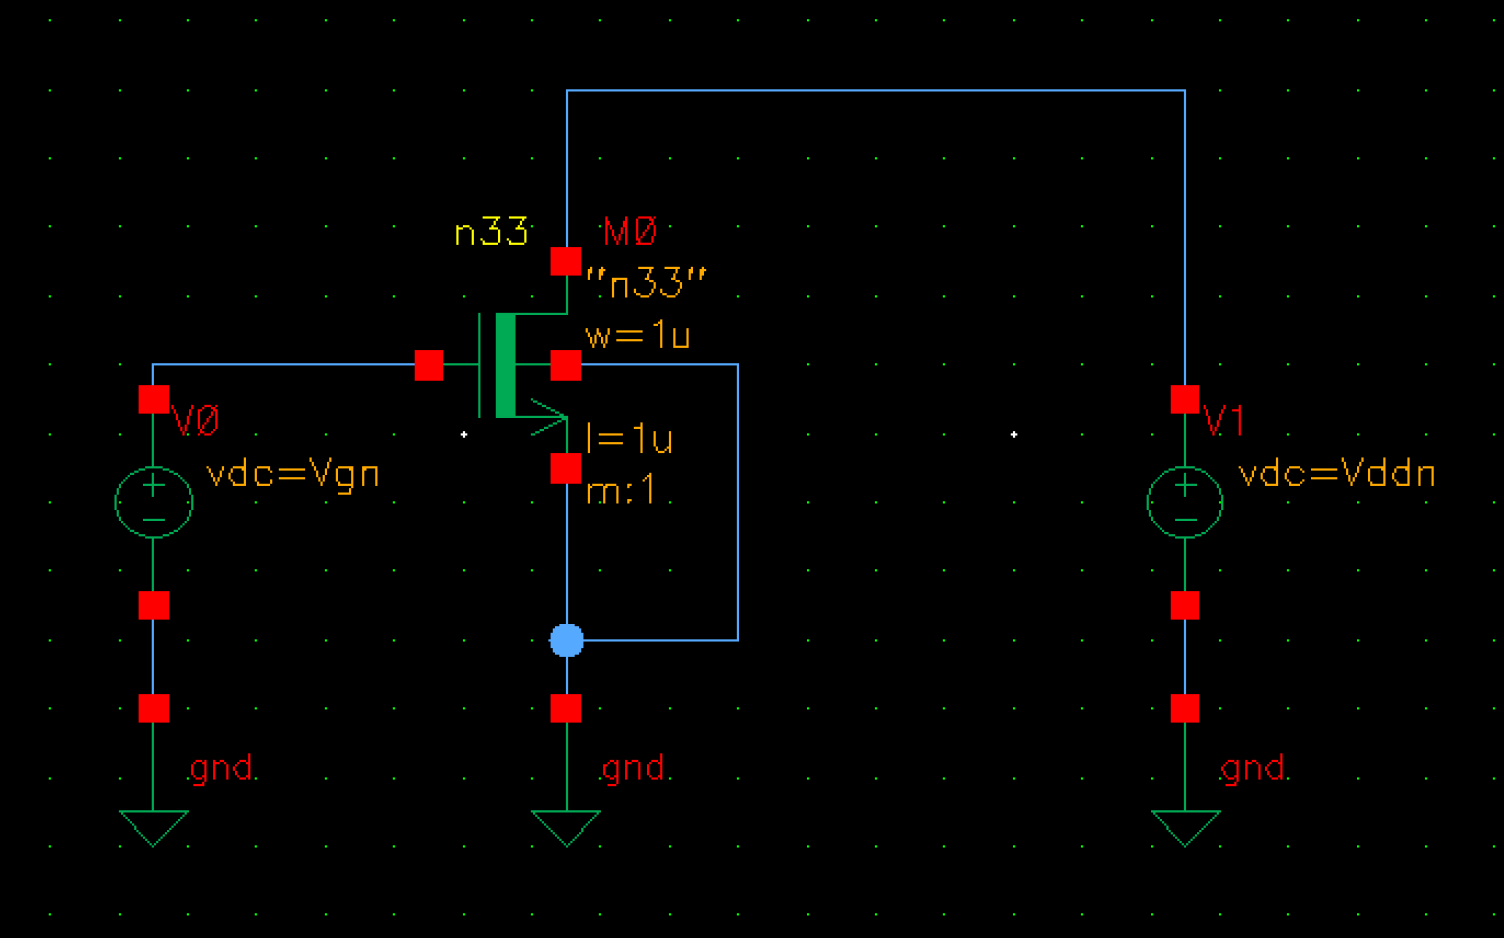
\includegraphics[width=0.8\textwidth]{NMOS_parameter.png}
    \end{center}
    \caption{NMOS管参数测量电路}
    \label{NMOS parameter circuit}
\end{figure}

\begin{table}[!ht]
    \centering
    \begin{tabular}{l l}
    \toprule
        $T_{oxe}$ & \SI{6.65}{\nano\meter} \\ 
        $\mu_n$ & \SI{350}{{\centi\square\meter}\per{\volt\cdot\second}} \\ 
        $V_{th0}$ & \SI{695}{\milli\volt} \\ 
        $g_{ds}$ & \SI{336.983}{\nano\siemens} \\ \midrule
        $C_{ox}$ & \SI{5.19268}{\milli\farad\per{\square\meter}} \\ 
        $K^{'}_{n}$ & \SI{181.744}{\milli\ampere\per{\square\volt}} \\ 
        $\lambda$ & 0.05778 \\ 
    \bottomrule
    \end{tabular}
    \caption{NMOS管关键性能参数}
    \label{NMOS key parameters}
\end{table}

\subsection{PMOS 管}
与NMOS管同理,测量电路图如\ref{PMOS parameter circuit}所示,测量以及计算所得的PMOS管关键参数列在表\ref{PMOS key parameters}中。


\begin{figure}[H]
    \begin{center}
        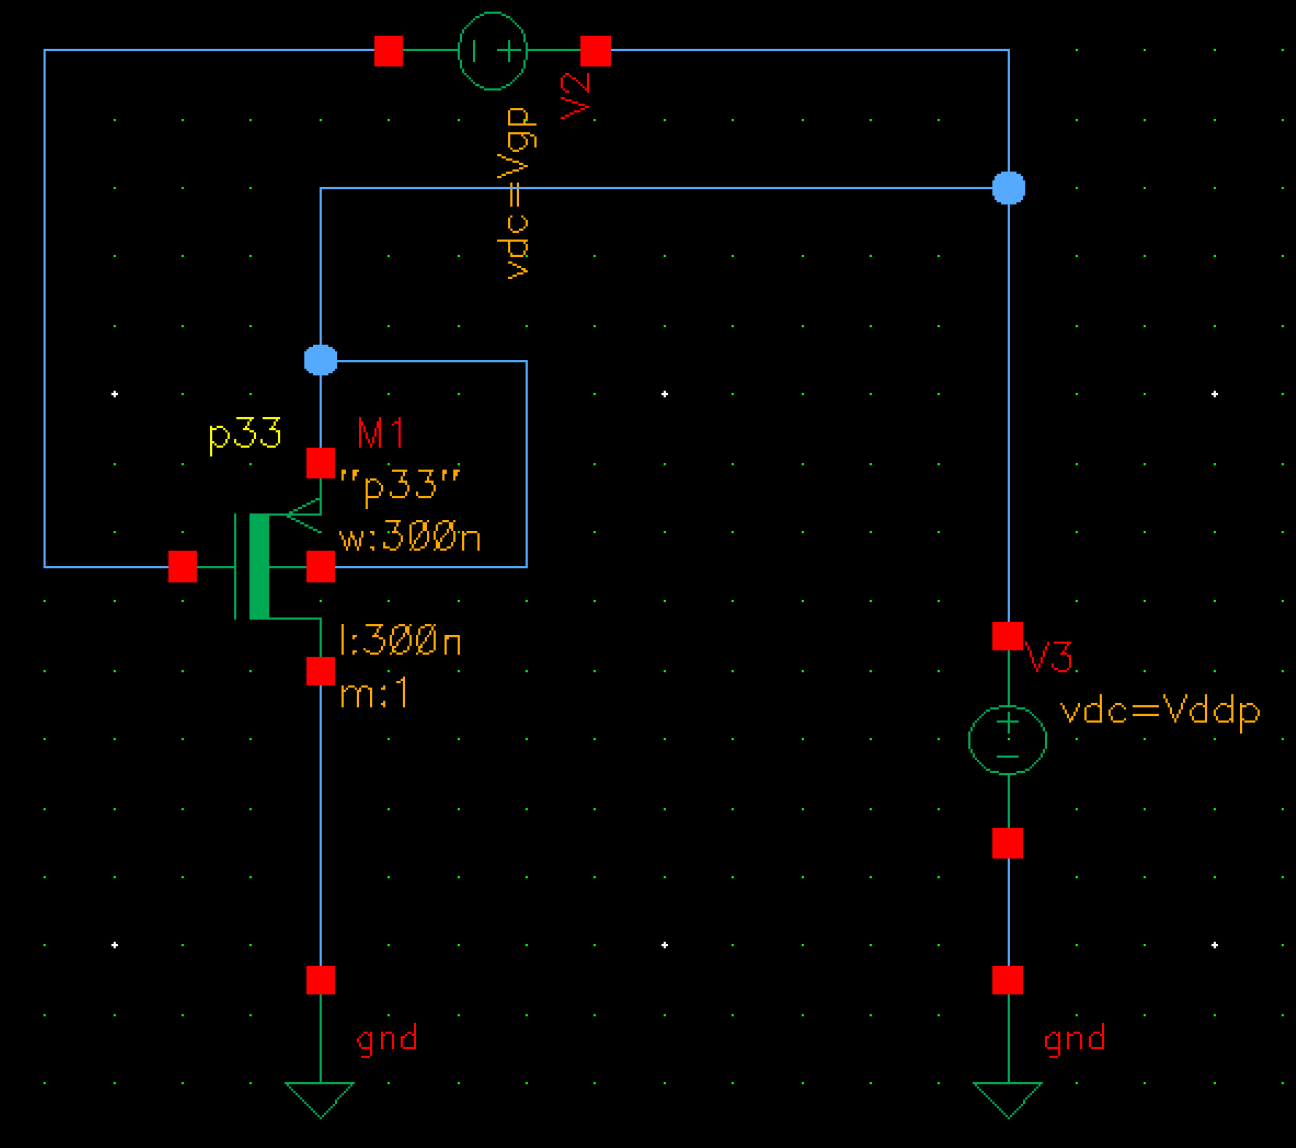
\includegraphics[width=0.8\textwidth]{PMOS_parameter.png}
    \end{center}
    \caption{PMOS管参数测量电路}
    \label{PMOS parameter circuit}
\end{figure}

\begin{table}[!ht]
    \centering
    \begin{tabular}{l l}
    \toprule
        $T_{oxe}$ & \SI{6.62}{\nano\meter} \\ 
        $\mu_n$ & \SI{92.5}{{\centi\square\meter}\per{\volt\cdot\second}} \\ 
        $V_{th0}$ & \SI{-672}{\milli\volt} \\ 
        $g_{ds}$ & \SI{230.227}{\nano\siemens} \\ \midrule
        $C_{ox}$ & \SI{5.21621}{\milli\farad\per{\square\meter}} \\ 
        $K^{'}_{n}$ & \SI{48.2499}{\milli\ampere\per{\square\volt}} \\ 
        $\lambda$ & 0.05676 \\ 
    \bottomrule
    \end{tabular}
    \caption{PMOS管关键性能参数}
    \label{PMOS key parameters}
\end{table}

\section{设计参数的确定}
\subsection{理论计算}
\subsubsection{运算放大器主体}
由于本次时间较为紧张,选用相对来讲更为简明的不带输出缓冲(unbuffered)的双级运算放大器结构。运算放大器整体结构如图\ref{op amp architecture}所示。

\begin{figure}[H]
    \begin{center}
        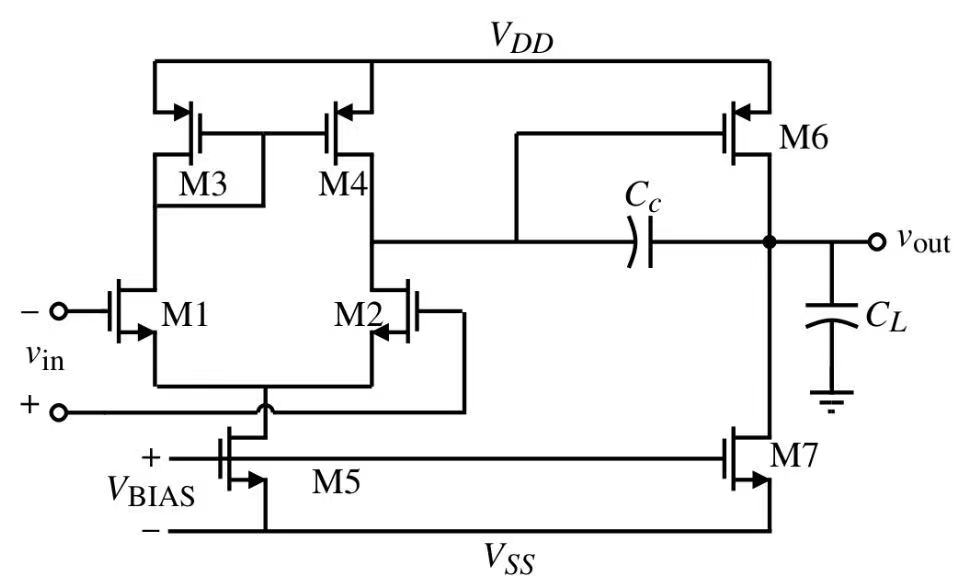
\includegraphics[width=0.8\textwidth]{op amp architecture.jpg}
    \end{center}
    \caption{选用的运算放大器整体结构}
    \label{op amp architecture}
\end{figure}

按顺序计算各参数如下:
\begin{enumerate}
    \item 选取沟道长度为\SI{1}{\micro\meter}
    \item 由\SI[]{60}{\degree}的相位裕量条件,要求\(C_c > 0.22\ C_l\),此处取\(C_c = \)\SI[]{3.3}{\pico\farad}
    \item 由压摆率限制,得最小的\(I_5 = SR \cdot C_c = \)\SI[]{9}{\micro\ampere}。此处取\(I_5 = \)\SI[]{10}{\micro\ampere}
    \item 要求的输入最高共模电压\SI[]{2.5}{\volt},取\(V_{inc,max} = \)\SI[]{3}{\volt},由\(\frac{2I_3}{K^{'}_{p} \left[ V_{dd} - V_{inc,max} - V_{tp} + V_{th} \right] ^{2}} = \) \SI[]{0.3}{\volt} 可得\(S_3 = S_4 = 2.138\)
    \item 由\(g_{m1} = GB \cdot C_c\),可得在单位增益带宽限制下,最小的\(g_{m1} = \)\SI[]{56.55}{\micro\siemens}。取\(g_{m1} = g_{m2} = \)\SI[]{80}{\micro\siemens}。则可得\(S_1 = S_2 = \frac{g_{m2}^{2}}{K^{'}_{n} I_5} = 3.52\)。
    \item 在输入最小共模电压约束下,\(V_{dsat5, max} = V_{inc,min} - V_{ss} - \sqrt{\frac{I_5}{K^{'}_N S_1}} - V_{thn} = \)\SI[]{0.43}{\volt}。取\(V_{dsat5} =\)\SI[]{0.3}{\volt},则有\(S_5 = \frac{2I_5}{K^{'}_N V_{dsat5}} = 1.22\)。
    \item 由相位裕量条件,\(g_{m6} > 2.2 g_{m2} \frac{C_L}{C_c}\),此处取\(g_{m6} = \)\SI[]{0.15}{\milli\siemens},由偏置的平衡条件,有\(V_{gs4} = V_{gs6}\),则\(S_6 = S_4 \frac{g_{m6}}{g_{m4}} = 7.99\)
    \item \(I_6 = \frac{g_{m6}^{2}}{2K_{p}^{'}S_6} = \)\SI[]{29.182}{\micro\ampere},由镜像电流源电流关系,\(S_7 = S_5 \frac{I_6}{I_5} = 3.56\)
    \item 验证输出级的饱和压降满足输出范围要求
    \item 验证\(A_v = \frac{2g_{m2}g_{m6}}{I_5 I_6 (\lambda_p + \lambda_n)^2} = 6269.19\)、\(P_{diss} = (I_5 + I_6)V_{dd} = \)\SI{129.29}{\micro\watt}均满足设计要求
\end{enumerate}

\subsubsection{偏置电流源}
由于本次时间较为紧张,且对于不含折叠共源共栅结构的运算放大器结构来说,单级镜像电流源已经能够满足性能需求,故采用如图\ref{current source circuit}的电路结构。

\begin{figure}[!ht]
    \begin{center}
        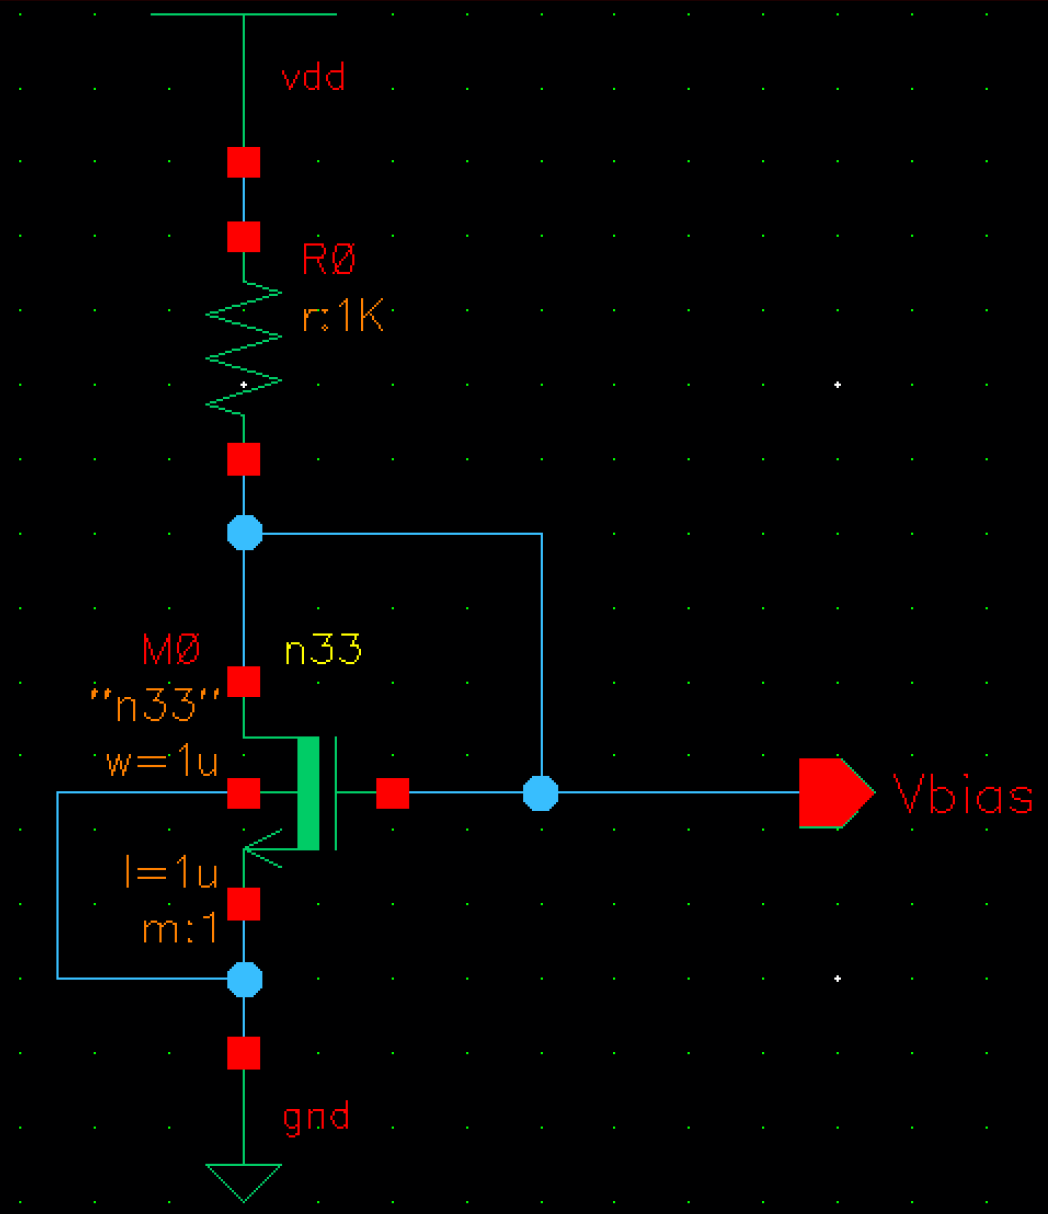
\includegraphics[width=0.5\textwidth]{Vbias.png}
    \end{center}
    \caption{偏置电流源结构}
    \label{current source circuit}
\end{figure}

通过\(I_5,\ S_5\)可以反推出$V_{gs5} = $ \SI[]{0.995}{\volt}。由

\begin{equation}
\left\{
\begin{aligned}
    & I_d = \frac{1}{2}K^{'}_{N}\cdot 1 \cdot \left(V_{gs} - V_{th}\right)^2 \\
    & V_{gs} = V_{dd} - I_d \cdot R\\
\end{aligned}
\right.
\end{equation}

可以解得\(I_d = \) \SI[]{8.18}{\micro\ampere}, \(R = \) \SI[]{281.8}{\kilo\ohm}

\subsection{参数调整}

\subsubsection{仿真中遇到的问题}
在Cadence中搭建电路并仿真后,主要遇到了以下问题:
\begin{enumerate}
    \item 推测可能是由于电路中存在其他寄生电容的原因,仿真时按照如上过程选取的一组参数无法达到\SI[]{45}{\degree}相位裕量的要求。
    \item 可能是由于存在细微误差的原因,输出级未能处于正常偏置状态。
\end{enumerate}

\subsubsection{整体调整思路}
针对以上问题,对电路参数做了以下调整:
\begin{enumerate}
    \item 增大\(C_c\),保证充足的相位裕量。
    \item 增大\(I_5\),保证有足够的压摆率。
    \item 增大\(S_1,\ S_2\),抵消掉\(I_5\)增大带来的增益下降,同时保证有足够的单位增益带宽\(GB\)。
    \item 调整\(S_3,\ S_4\),使得差分级处于正常的偏置状态。
    \item 调整\(S_6,\ S_7\),增大增益并使输出级正常偏置。
\end{enumerate}


\subsection{参数确定}
经过一系列结合仿真结果的调整后,最终确定设计如\ref{design circuit}所示,其中的各参数整理在表\ref{design parameters}中。

\begin{figure}[!ht]
    \begin{center}
        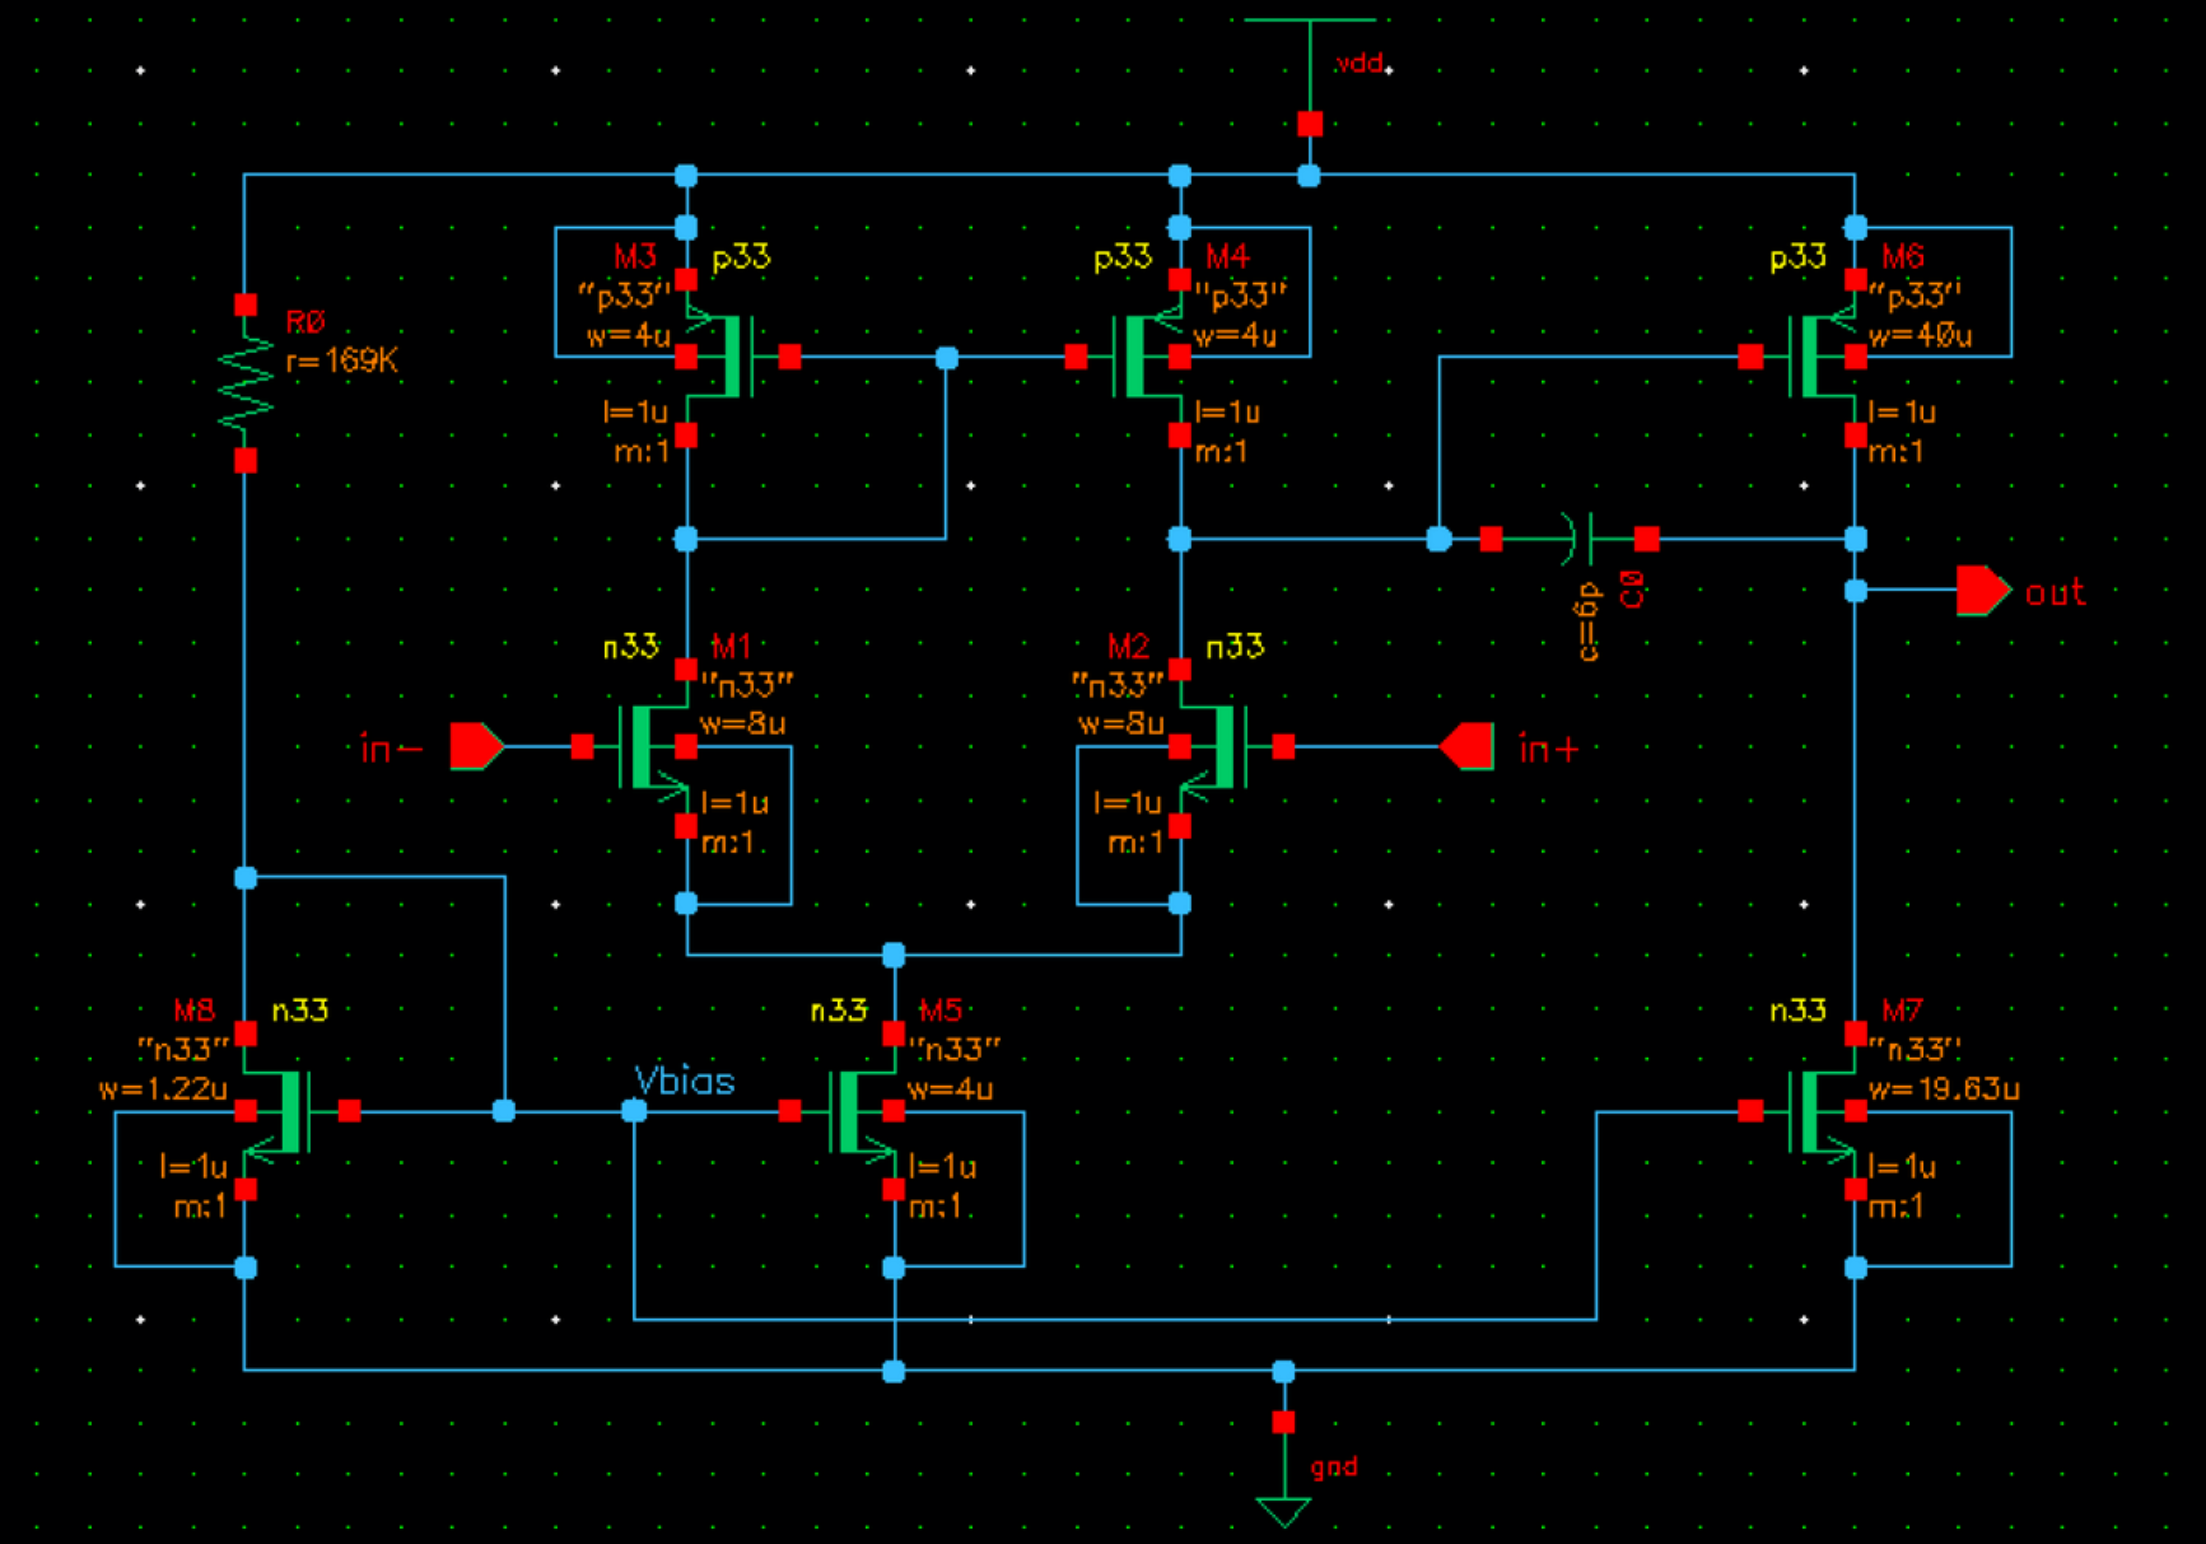
\includegraphics[width=0.9\textwidth]{design circuit.png}
    \end{center}
    \caption{运算放大器电路}
    \label{design circuit}
\end{figure}

\begin{table}[!ht]
    \centering 
    \begin{tabular}{l l}
    \toprule
        $S_1$ & 8\\ 
        $S_2$ & 8\\ 
        $S_3$ & 4\\ 
        $S_4$ & 4\\ 
        $S_5$ & 4\\ 
        $S_6$ & 40\\ 
        $S_7$ & 19.63\\
        $S_8$ & 19.63\\
        $C_c$ & \SI[]{6}{\pico\farad}\\
        $R_0$ & \SI[]{169}{\kilo\ohm}\\
    \bottomrule
    \end{tabular}
    \caption{设计参数}
    \label{design parameters}
\end{table}

\section{运算放大器仿真及性能测试}

\subsection{瞬态响应}
仿真电路、仿真设定与仿真结果均展示在图\ref{trans simulation}中。可以看到,输出电压振荡中心大约在\SI{1.65}{\volt}处,且正弦波形无明显失真,说明运算放大器整体工作正常,能够起到放大作用。由输入电压振幅\SI[]{10}{\micro\volt},输出电压振幅\SI[]{0.53}{\volt},可以得到准静态状态下的\(A_v = 50344\),远高于设计要求。

\begin{figure}[H]
    \centering
    \subfigure[仿真电路]{
    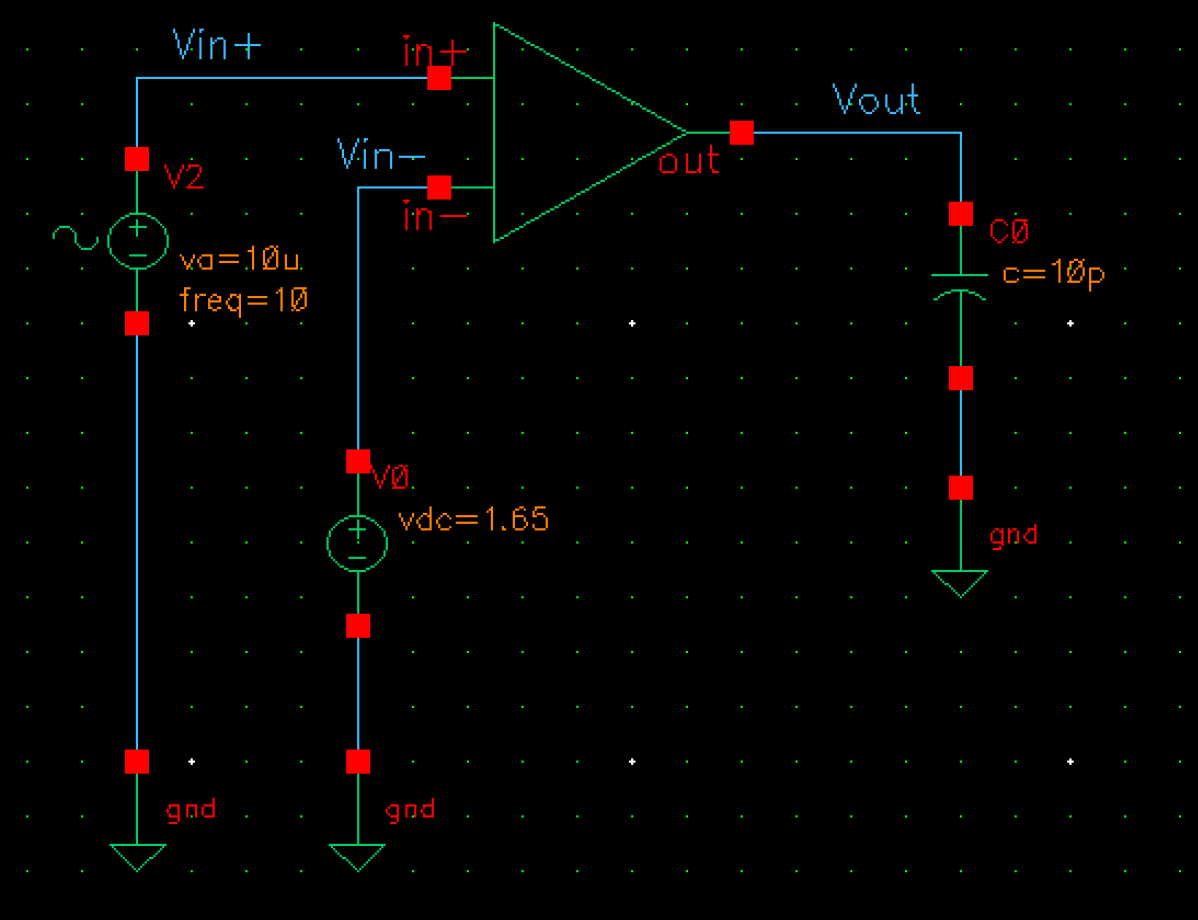
\includegraphics[width=0.53\textwidth]{trans/circuit.png}}
    \subfigure[仿真设定]{
    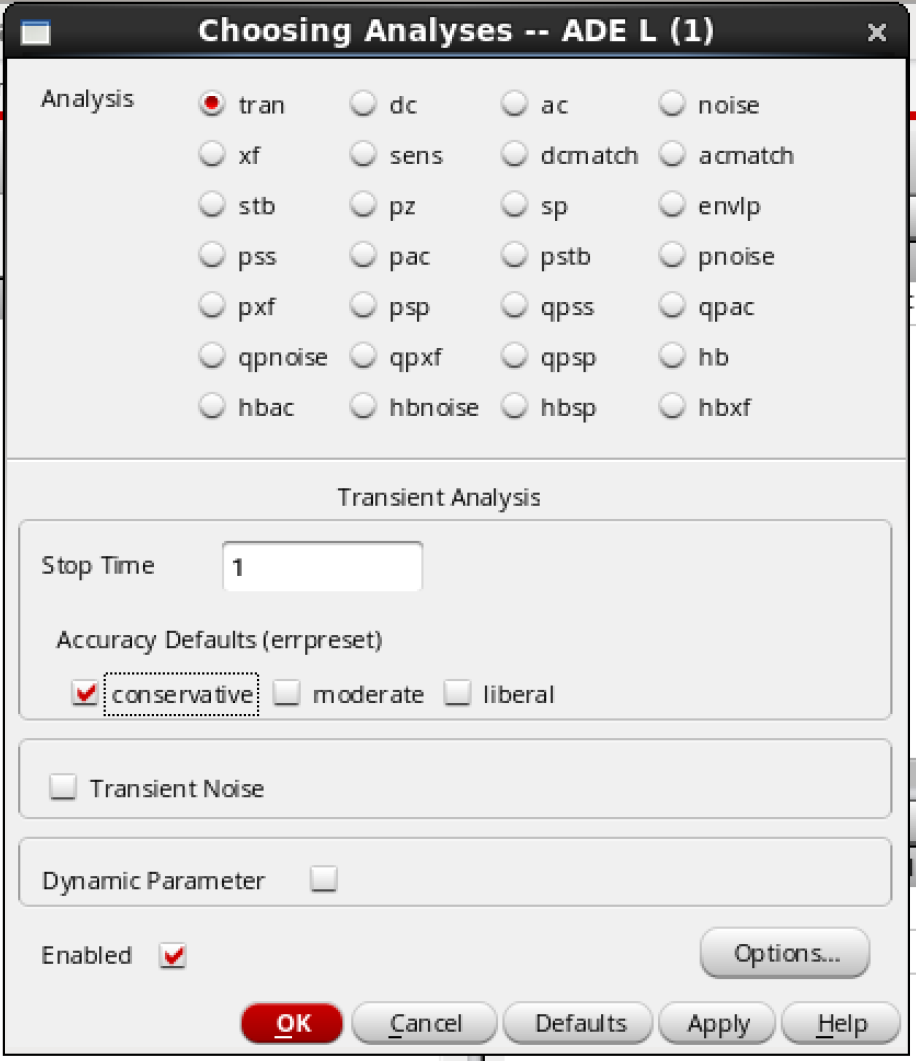
\includegraphics[width=0.35\textwidth]{trans/sim settings.jpg}}
    \subfigure[仿真结果]{
    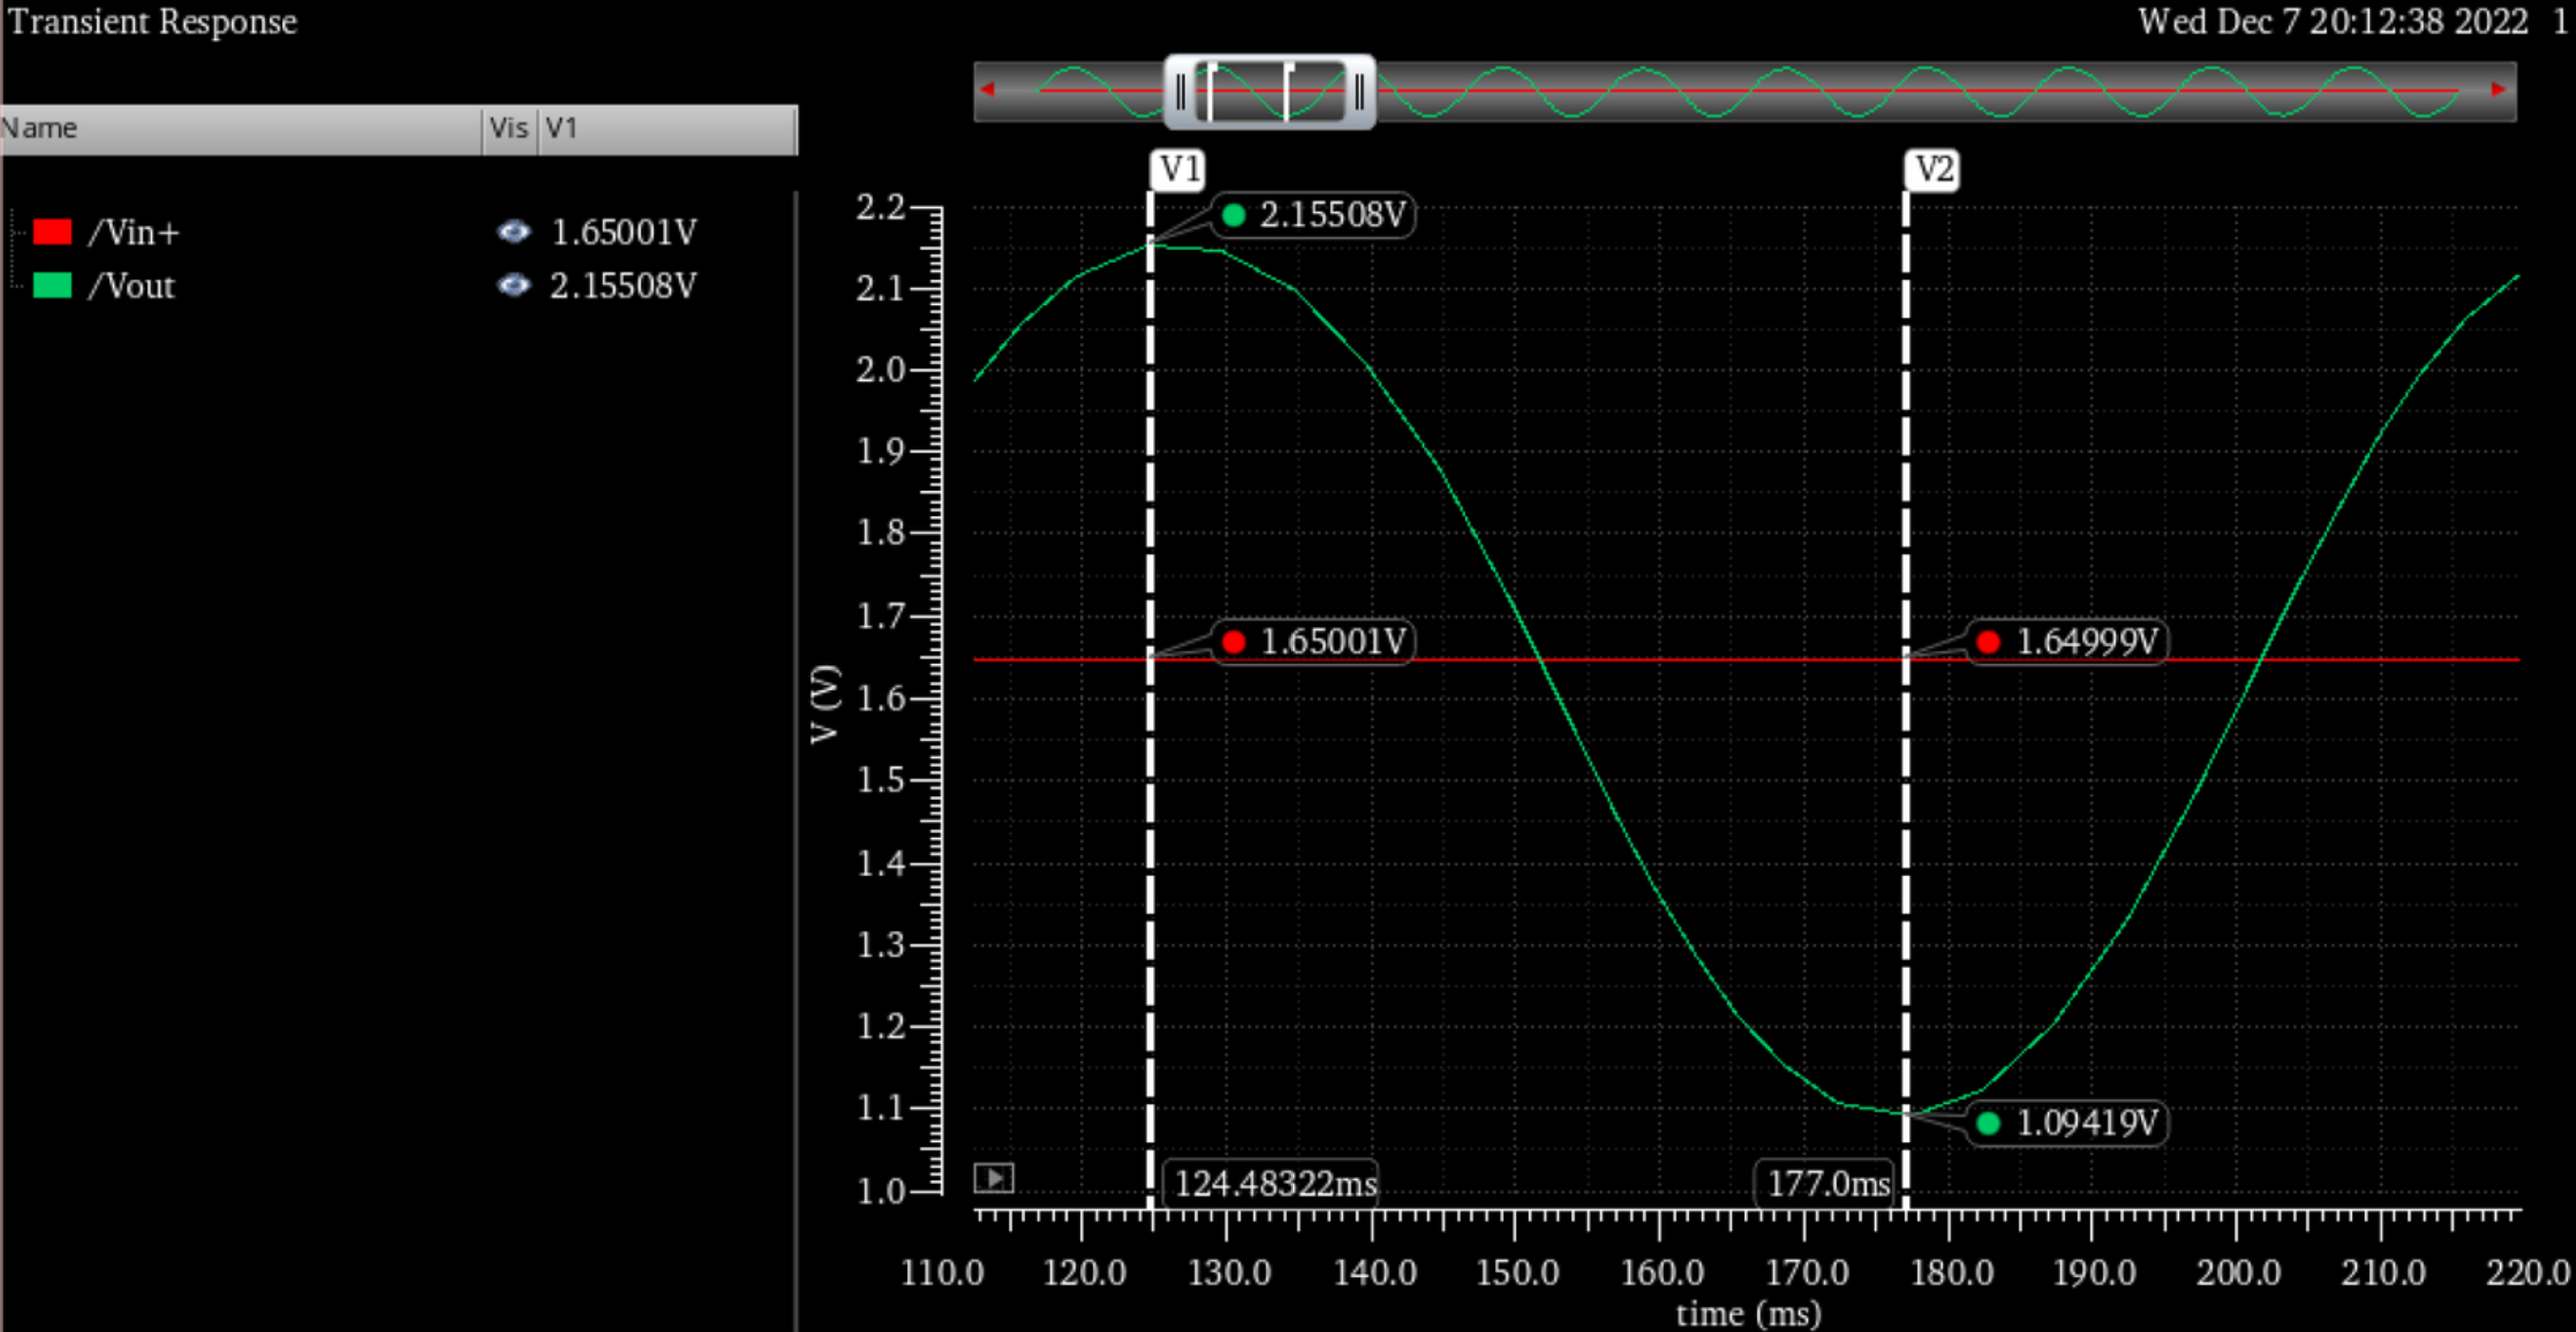
\includegraphics[width=0.9\textwidth]{trans/sim result.png}}
    \caption{仿真:瞬态响应}
    \label{trans simulation}
\end{figure}

\subsection{传输特性曲线 电压输出范围}
仿真电路及仿真结果展示在图\ref{transfer simulation}中。仿真结果中同时选取了电路中一些关键节点进行画图。可以看到,运算放大器正常工作时,所有MOS均正常偏置,工作在饱和区。

同时,对于要求的输出范围:
\begin{enumerate}
    \item 当\(V_{out} = \) \SI{0.4}{\volt}时,\(V_{g7} = V_{bias} = \) \SI[]{1.1073}{\volt},\(V_{s7}  = \) \SI[]{0}{\volt},\(V_{d7} = V_{out} =\) \SI[]{0.4}{\volt},\(V_{th}  = \) \SI[]{695}{\milli\volt}。关系\(V_{ds} > V_{gs} - V_{th}\)成立,工作在饱和区。
    \item 当\(V_{out} = \) \SI{2.6}{\volt}时,\(V_{g6} = \) \SI[]{2.0828}{\volt},\(V_{s6}  = \) \SI[]{3.3}{\volt},\(V_{d6} = V_{out} =\) \SI[]{2.6}{\volt},\(V_{th}  = \) \SI[]{672}{\milli\volt}。关系\(|V_{ds}| > |V_{gs}| - |V_{th}|\)成立,工作在饱和区。
\end{enumerate}

\begin{figure}[H]
    \centering
    \subfigure[仿真电路]{
    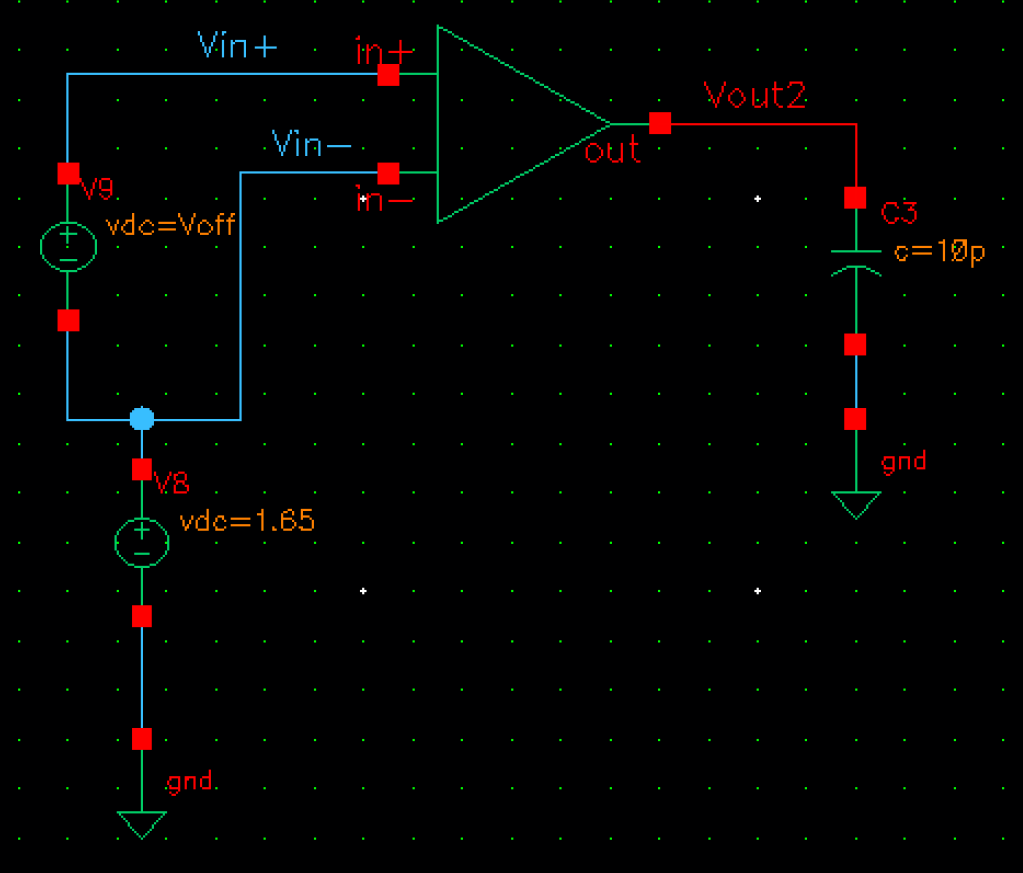
\includegraphics[width=0.55\textwidth]{transfer/circuit.png}}
    \subfigure[仿真结果 - \(V_{out,min}\)]{
    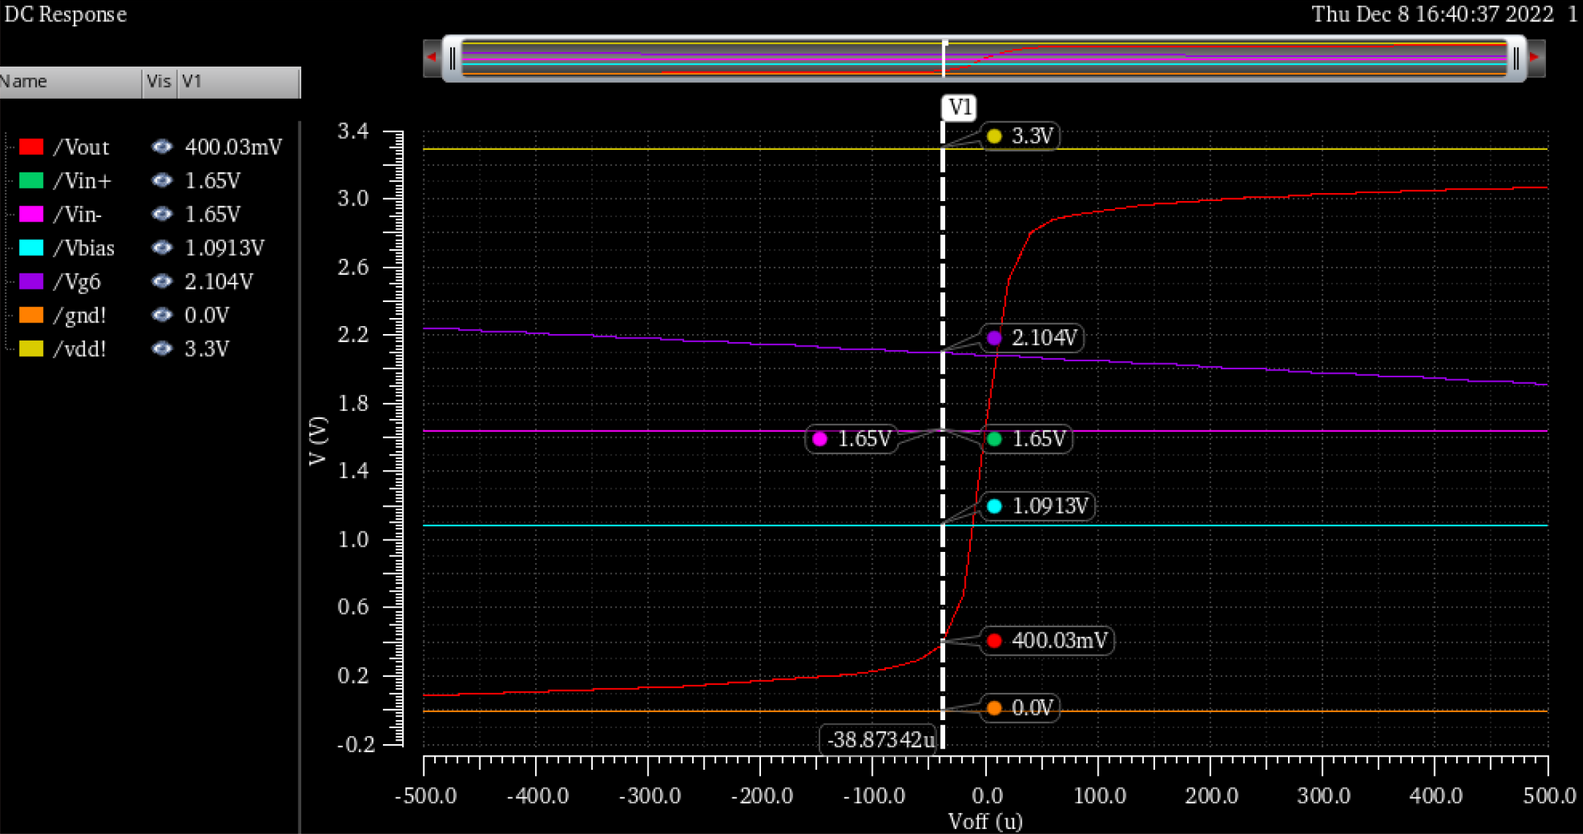
\includegraphics[width=0.45\textwidth]{transfer/res1.png}}
    \subfigure[仿真结果 - \(V_{out,max}\)]{
    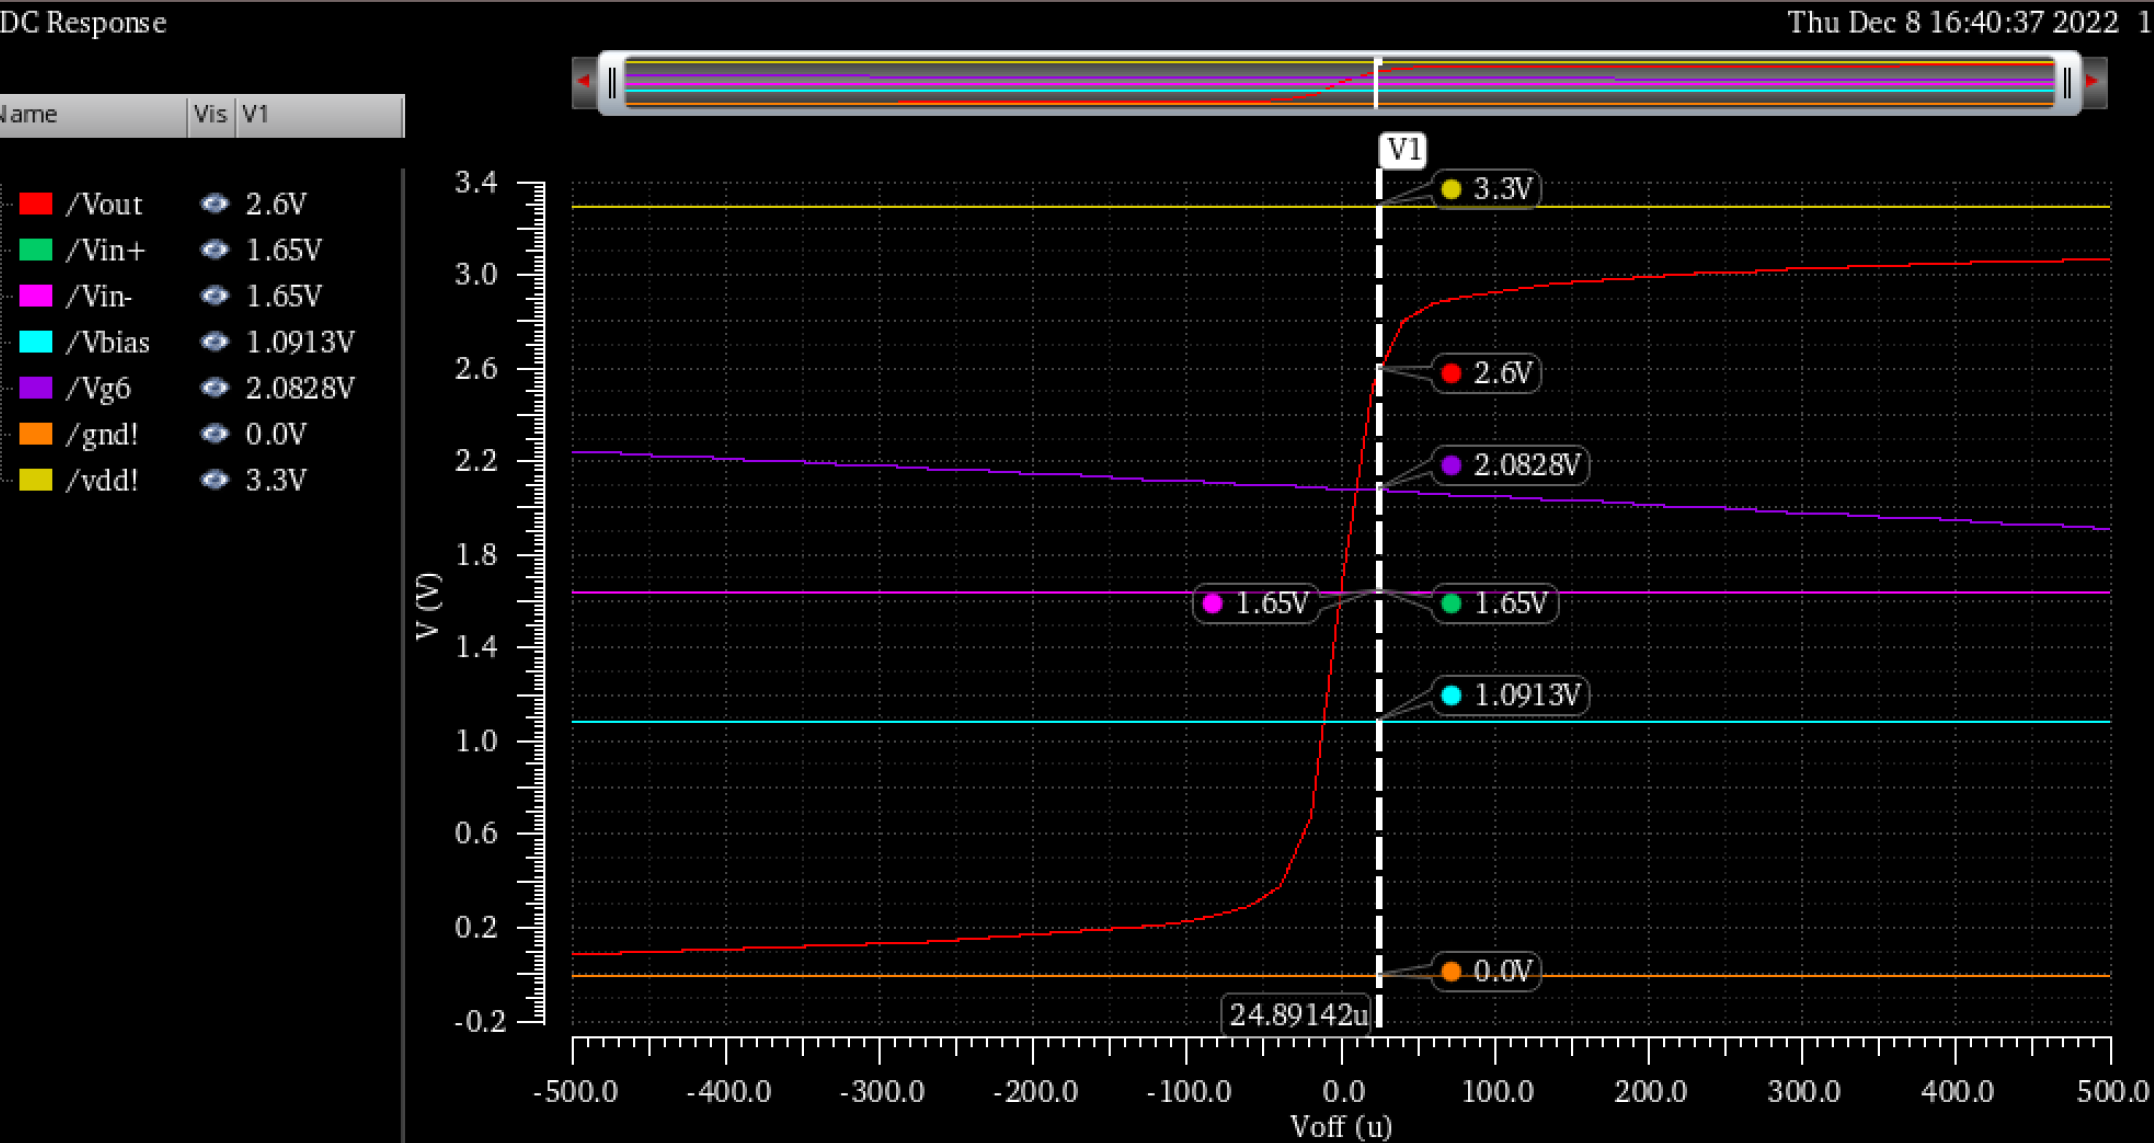
\includegraphics[width=0.45\textwidth]{transfer/res2.png}}
    \caption{仿真:瞬态响应}
    \label{transfer simulation}
\end{figure}

\subsection{频率响应}
仿真电路及仿真结果展示在图\ref{AC simulation}中。可以看到,静态时增益\SI[]{95.207}{\dB} \( = 57590\),远超设计标准。相位裕量\(\varphi_m = \) \SI[]{47.01}{\degree},满足设计标准。单位增益带宽\(GB = \) \SI[]{5.31657}{\MHz},远超设计标准。

\begin{figure}[H]
    \centering
    \subfigure[仿真电路]{
    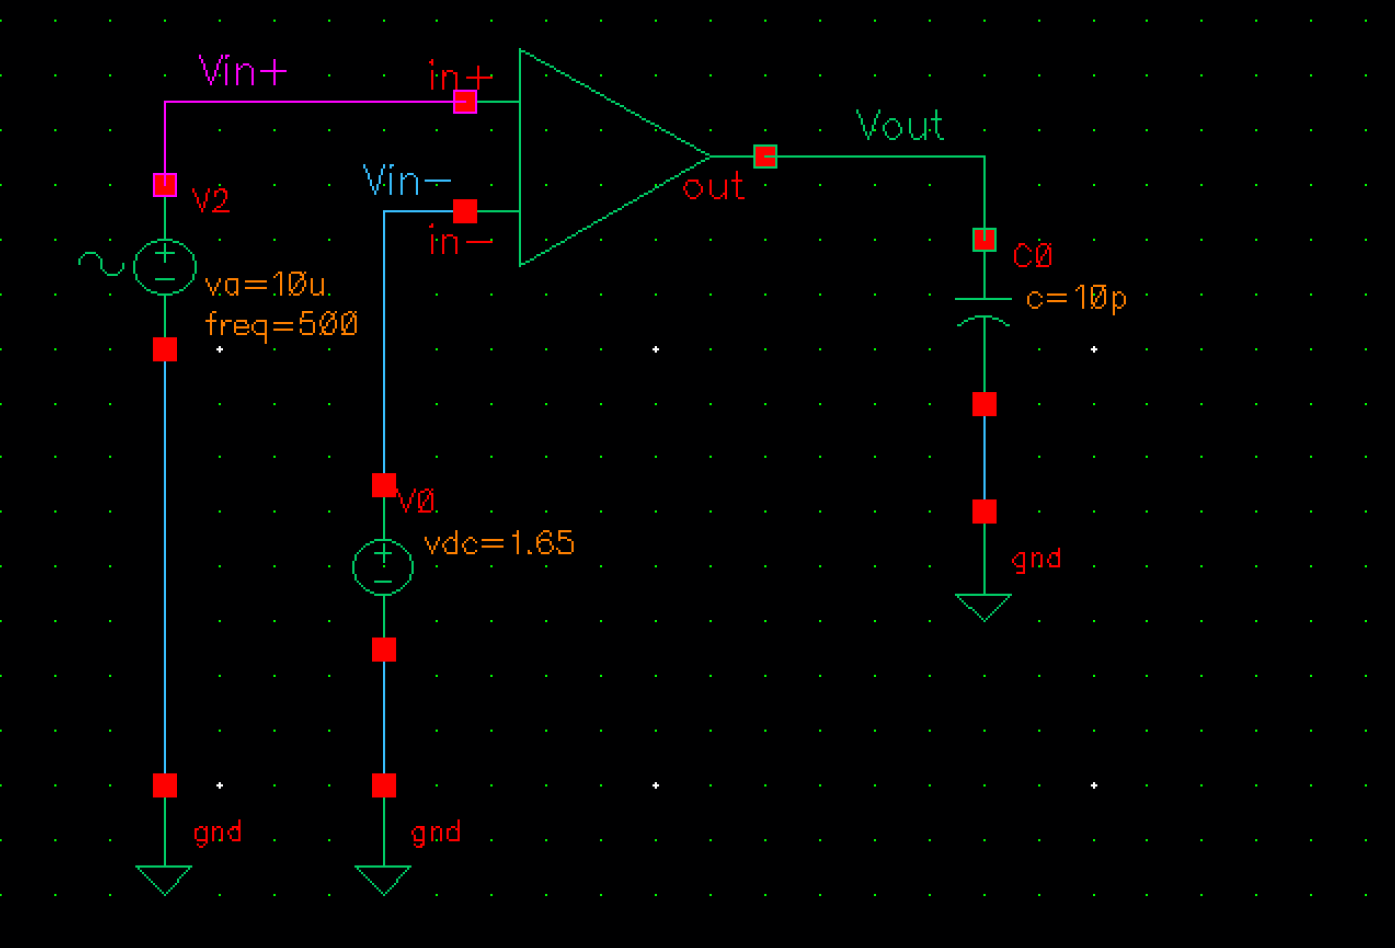
\includegraphics[width=0.45\textwidth]{AC/circuit.png}}
    \subfigure[相位裕量计算结果]{
    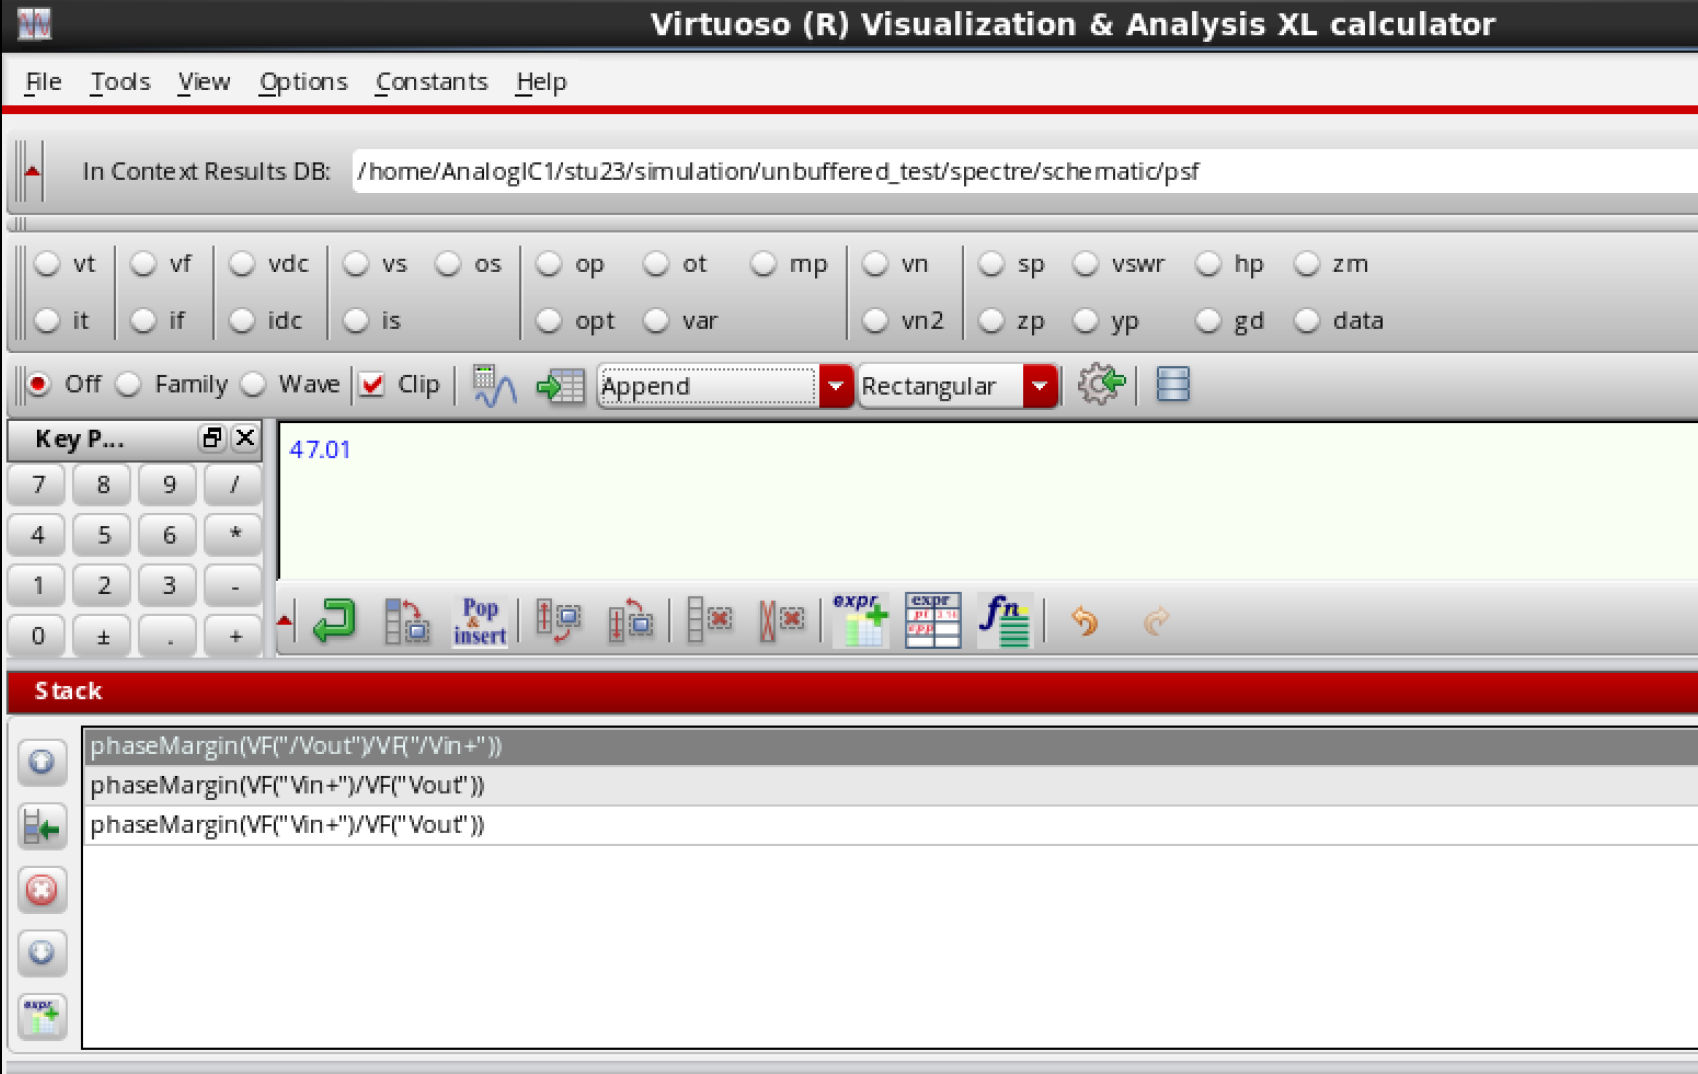
\includegraphics[width=0.45\textwidth]{AC/phi_m.png}}
    \subfigure[仿真结果 - \(A_{v0}\)]{
    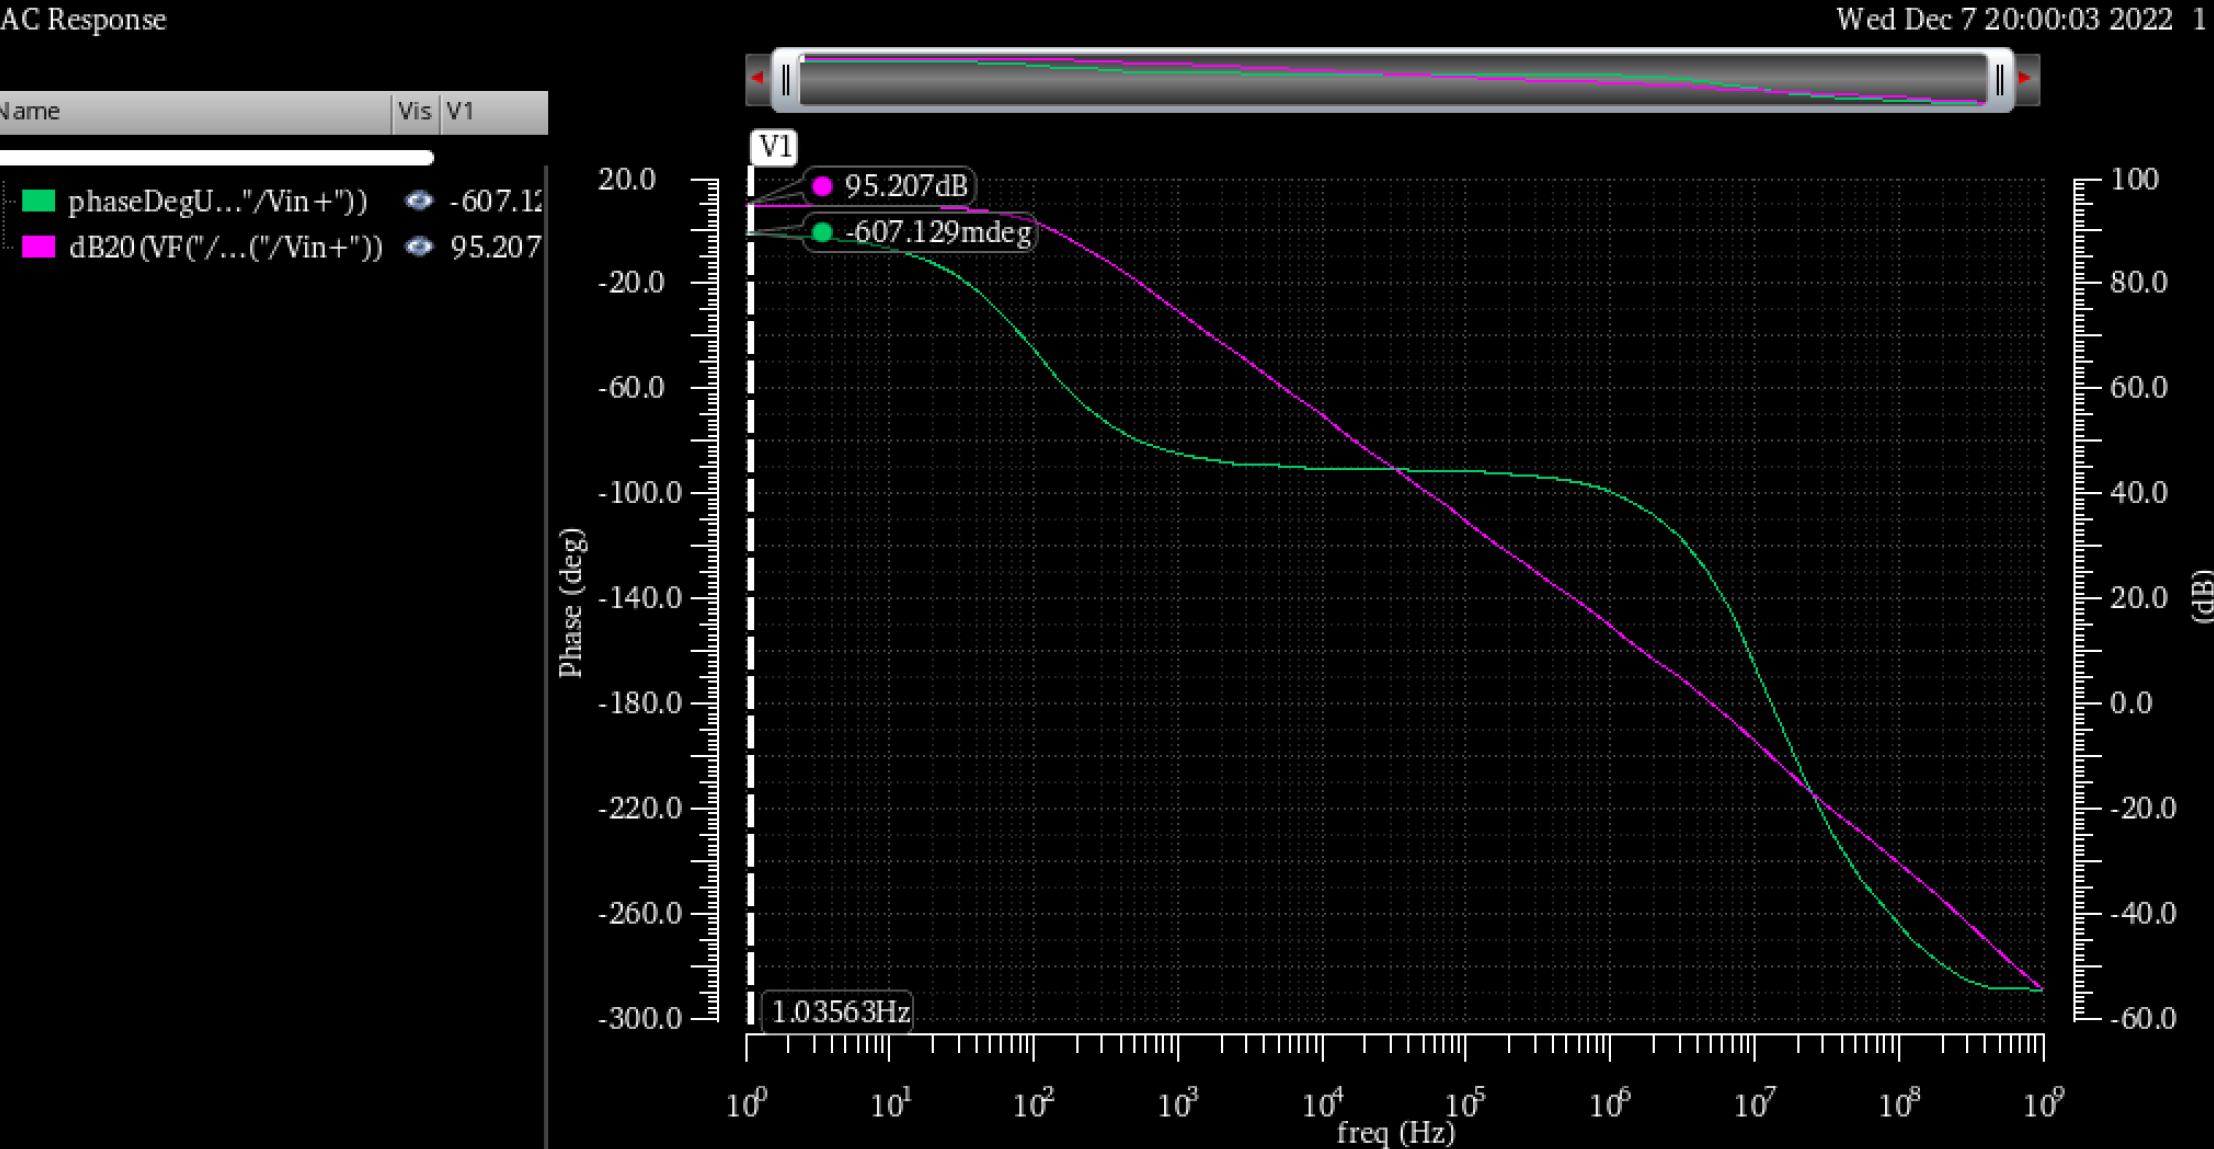
\includegraphics[width=0.45\textwidth]{AC/res2.png}}
    \subfigure[仿真结果 - \(\varphi_m\)]{
    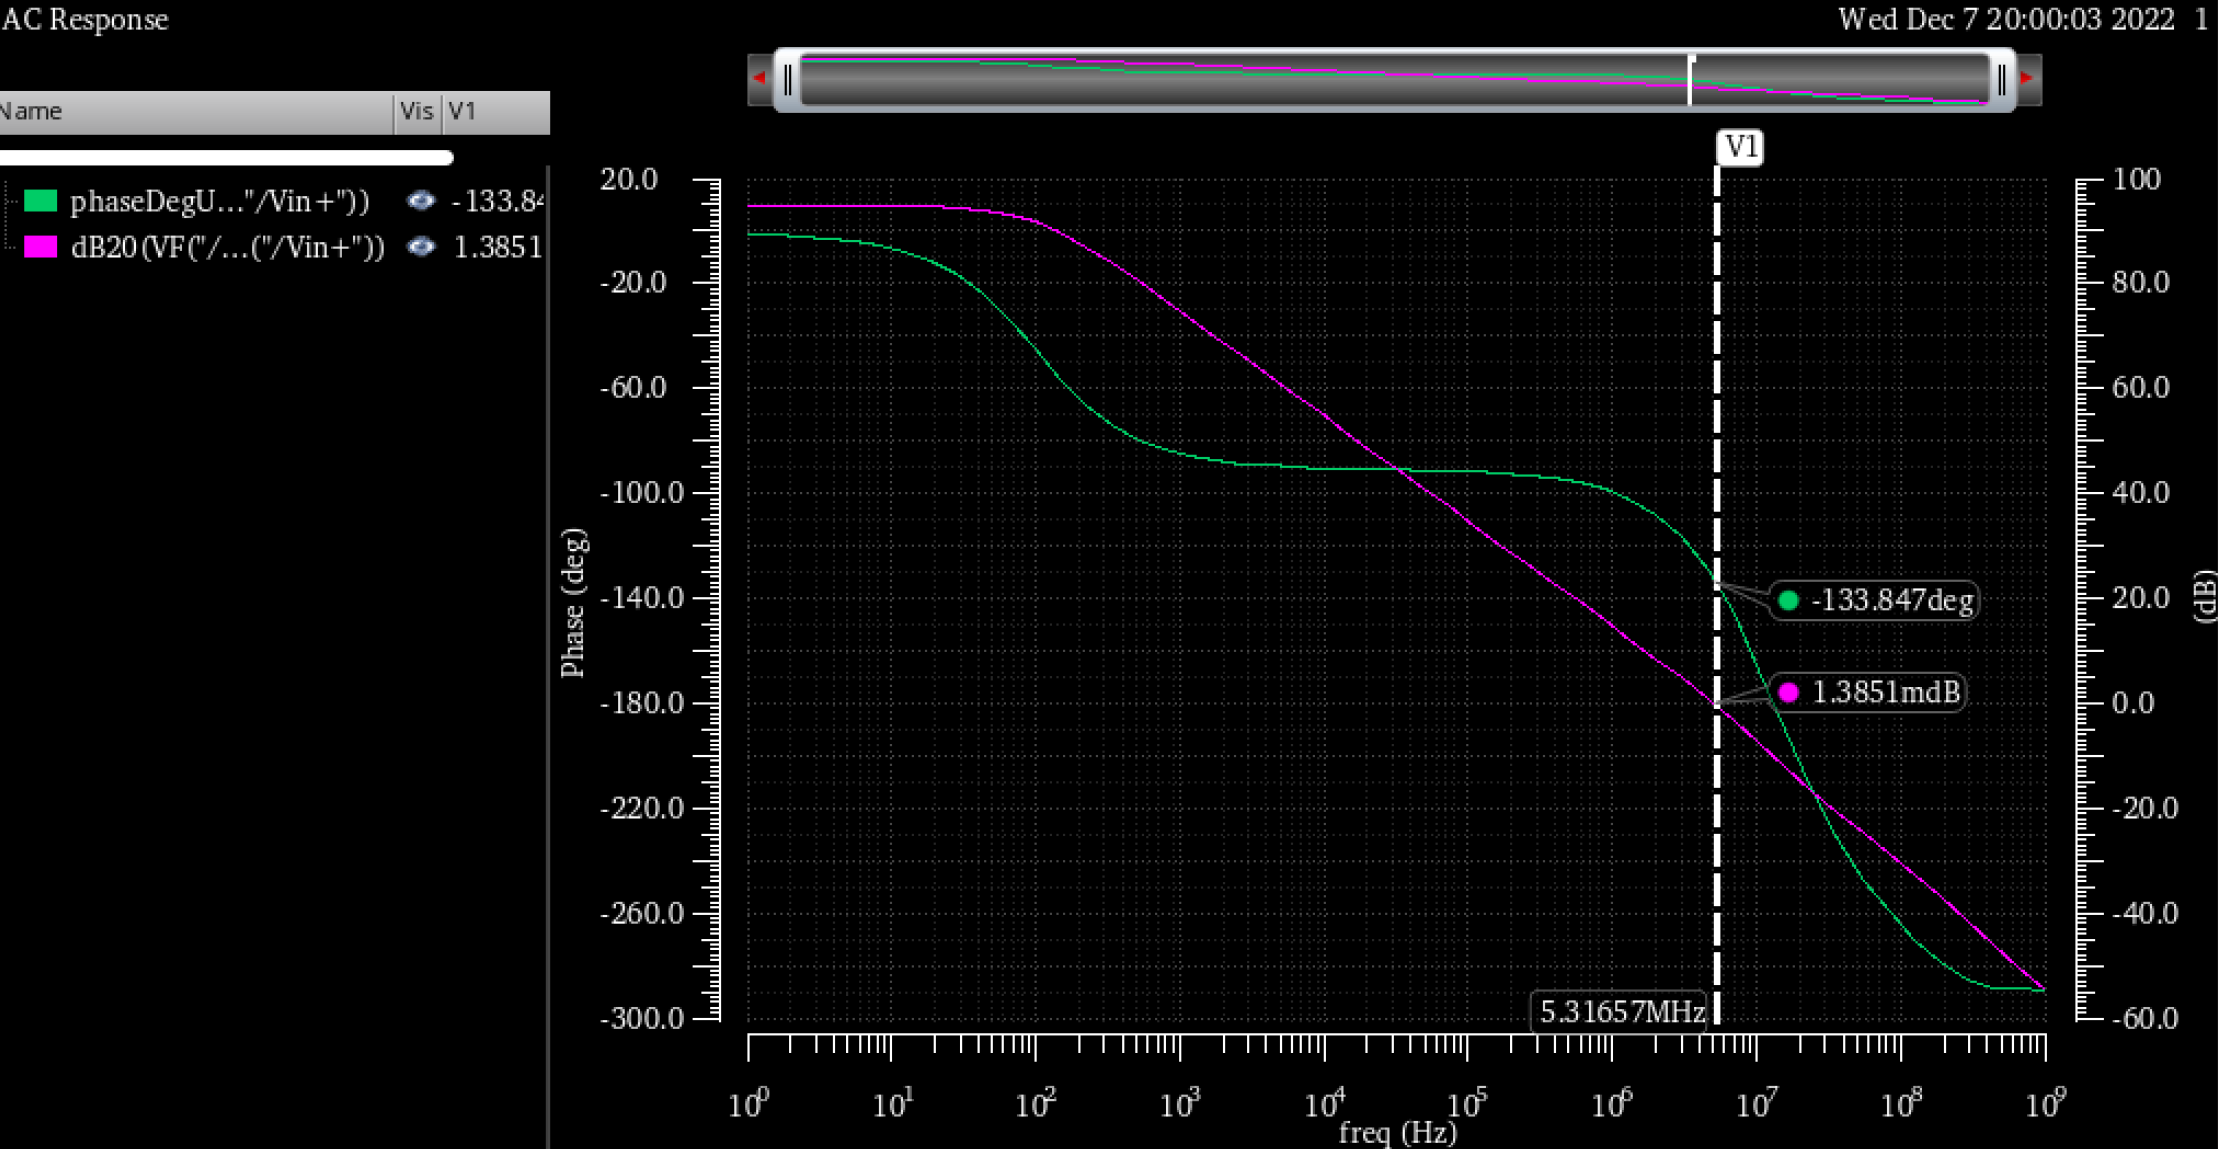
\includegraphics[width=0.45\textwidth]{AC/res1.png}}
    \caption{仿真:频率响应}
    \label{AC simulation}
\end{figure}

\subsection{共模抑制比 CMRR}
\subsubsection{闭环测试方案}
仿真电路及仿真结果展示在图\ref{AC simulation}中。由电路连接方式,则有关系
\[\frac{V_{cm}}{V_{out}} = \pm \frac{1+A_v \mp \frac{A_c}{2}}{A_c} \simeq \frac{A_v}{|A_c|} = CMRR\]

\begin{figure}[H]
    \centering
    \subfigure[仿真电路]{
    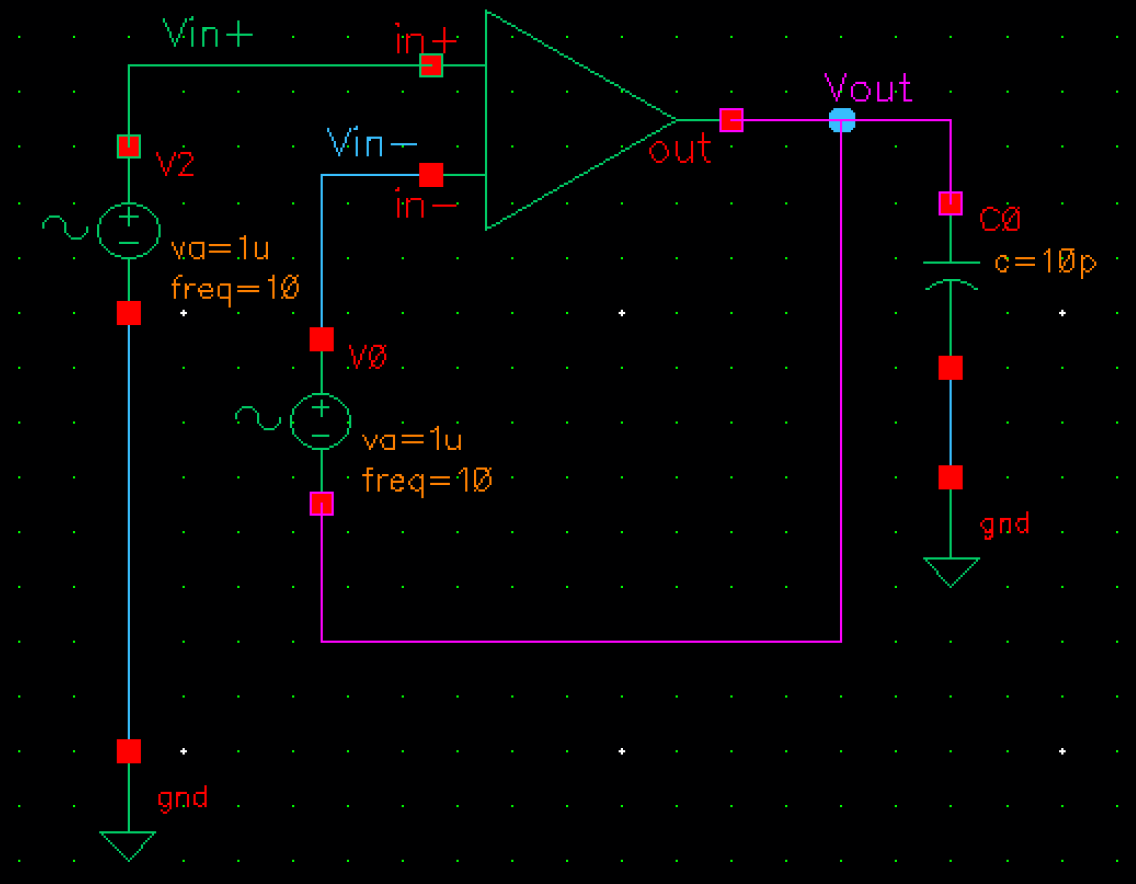
\includegraphics[width=0.35\textwidth]{CMRR/close/circuit.png}}
    \subfigure[仿真结果 ]{
    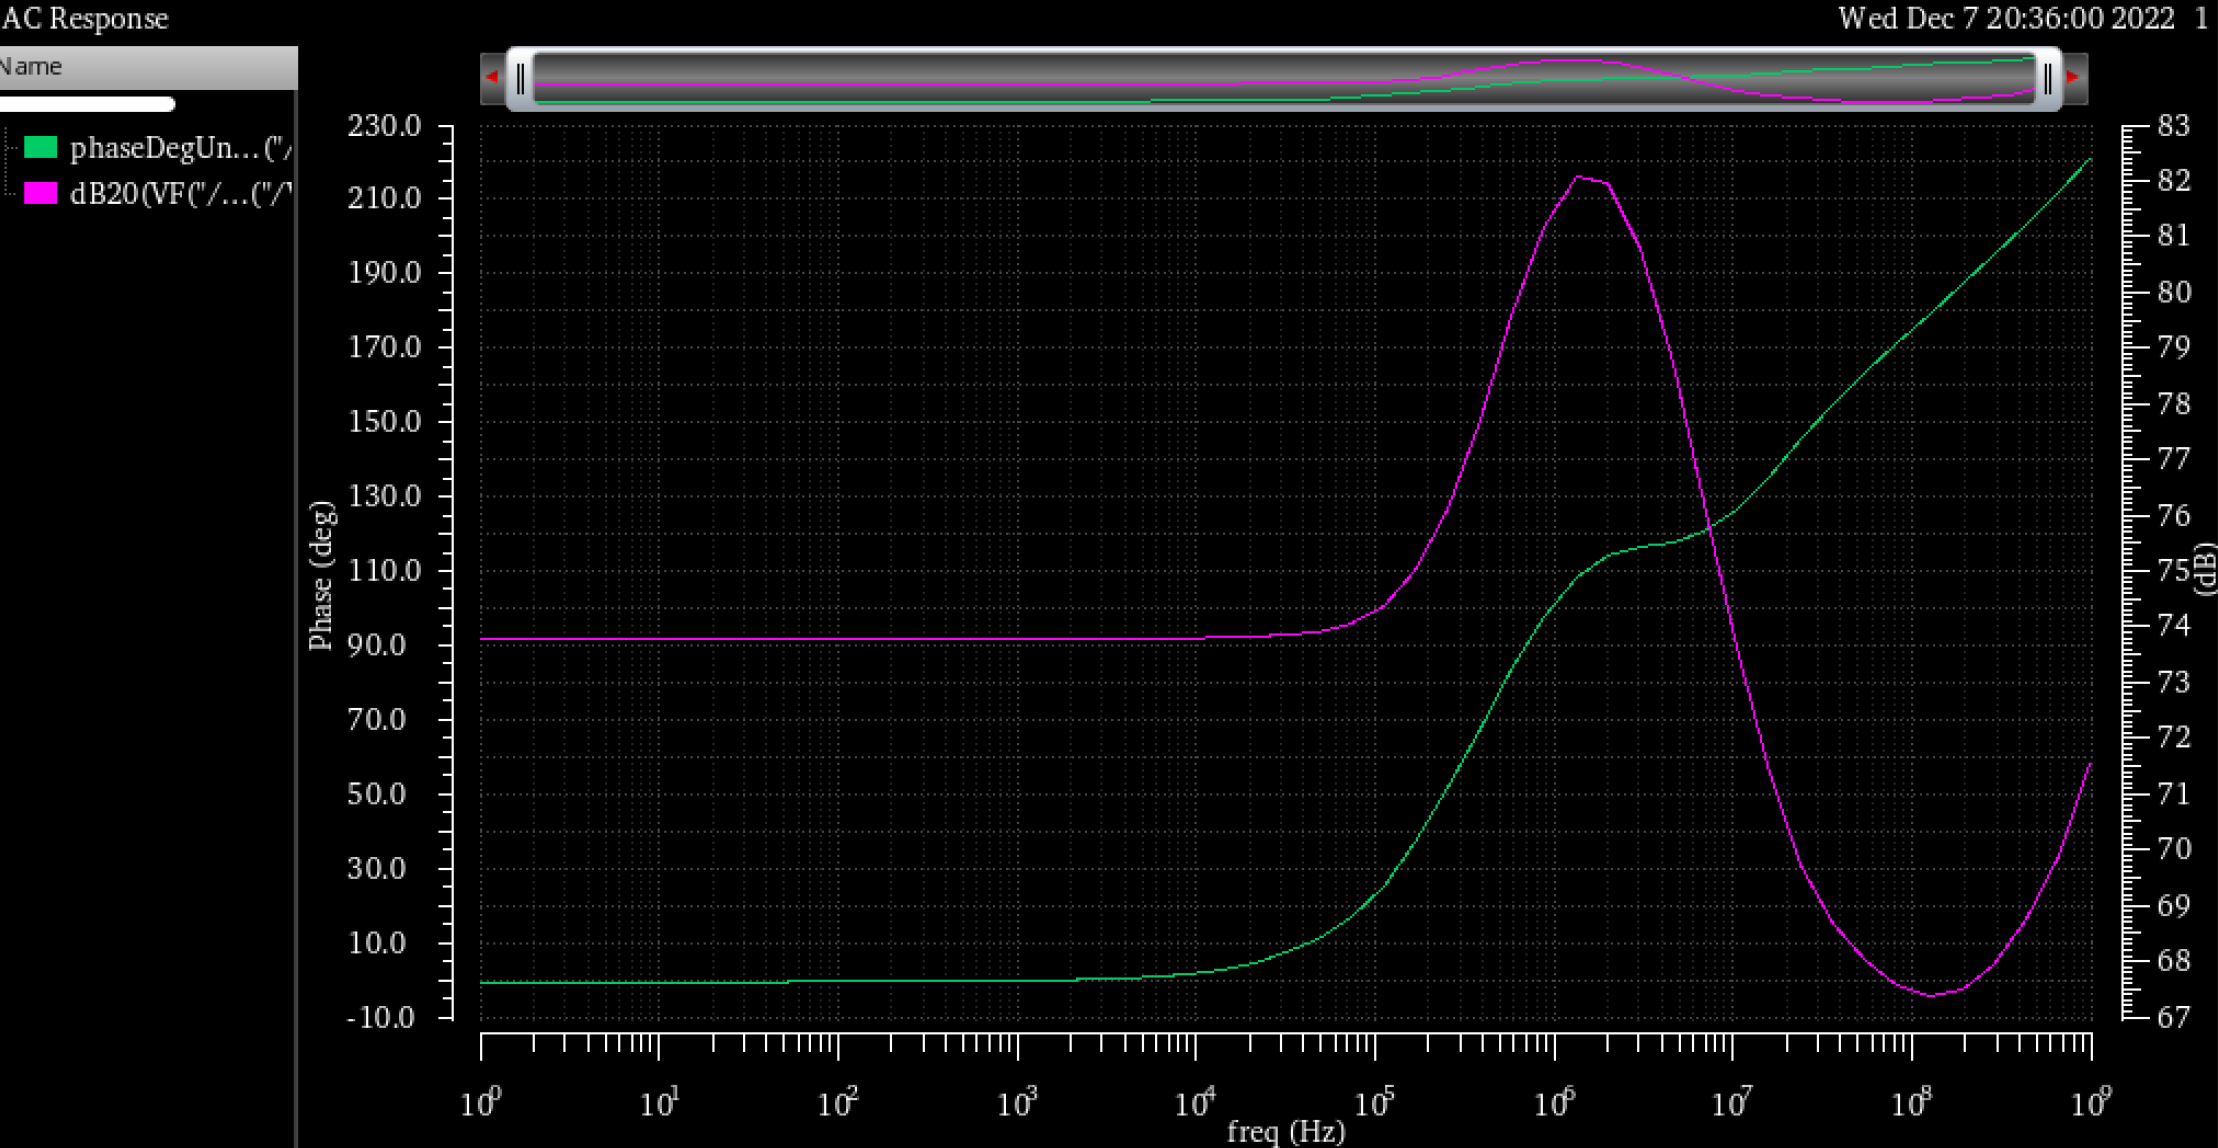
\includegraphics[width=0.55\textwidth]{CMRR/close/result.png}}
    \caption{仿真:共模抑制比 闭环测法}
    \label{CMRR closed simulation}
\end{figure}



\end{document}